\documentclass[12pt]{article}

%%%%%%%%%%%%
%%%% PACKAGE
%%%%%%%%%%%%
\usepackage[T1]{fontenc} 
\usepackage[utf8]{inputenc}
%\usepackage[frenchb]{babel}
\usepackage{times}
\usepackage{mltex}
\usepackage{xcolor}
\usepackage{url}
\usepackage{array}
\usepackage{epsfig}
\usepackage{subfigure}
\usepackage{lastpage}
\usepackage{fancyhdr,etoolbox}
\usepackage{ifthen}
\usepackage{fancyhdr,etoolbox}
\usepackage{titlesec}
\usepackage[usenames,dvipsnames]{pstricks}
\usepackage{thmbox}
\usepackage[
breaklinks,
colorlinks=true,
linkcolor=black,
urlcolor=black,
citecolor=black
]{hyperref}
\usepackage{enumitem}
\usepackage{amsfonts}
\usepackage{amsmath}
\usepackage{mathrsfs}
\usepackage{amsfonts}
\usepackage{graphicx}


%%%%%%%%%%%%
%%%% MARGING
%%%%%%%%%%%%
%\usepackage{geometry}
%\oddsidemargin = 21pt %31pt
%\topmargin = 0pt %20pt
%\headheight = 12pt
%\headsep = 25pt
%\textheight = 592pt
%\textwidth = 430pt %390pt
%\marginparsep = 10pt
%\marginparwidth = 35pt
%\footskip = 30pt
\usepackage[%
papersize={200mm,250mm},%
margin=2mm,%
includeheadfoot%
]{geometry}
\pagestyle{fancy}

%%%%%%%%%%%
%%%% HEADER
%%%%%%%%%%%
\renewcommand{\headrulewidth}{0.5pt}
\renewcommand{\footrulewidth}{0.0pt}
\makeatletter
\patchcmd{\@fancyhead}{\rlap}{\color{gray}\rlap}{}{}
\patchcmd{\headrule}{\hrule}{\color{gray}\hrule}{}{}
\patchcmd{\@fancyfoot}{\rlap}{\color{gray}\rlap}{}{}
\patchcmd{\footrule}{\hrule}{\color{gray}\hrule}{}{}
\makeatother

%\renewcommand{\footrulewidth}{0.5pt}
\fancyhead{}
\rhead{\textit{Emmanuel ROUBIN}}
\chead{}
\lhead{\today}
%\rfoot{page \thepage\ sur \pageref{LastPage}}
\rfoot{\thepage/\pageref*{LastPage}}
%\lfoot{\today}
\lfoot{}
\cfoot{}


%%%%%%%%%%
%%%% TITLE
%%%%%%%%%%
\newcommand{\maintitle}[2][YYY]{%
  \ifthenelse { \equal {#1} {YYY} }
              { \chead{#2} }
              { \chead{#1} }
  \begin{center}
    \textsc{\Large #2}
    \par\vspace{0.5cm}
  \end{center}
}

%%%%%%%%%%%%
%%%% SECTION
%%%%%%%%%%%%
%\renewcommand{\thesection}{\Roman{section}}
%\renewcommand{\thesubsection}{\Roman{subsection}}
%\renewcommand{\thesubsubsection}{\arabic{subsubsection}}
%\titleformat{⟨command⟩}[⟨shape⟩]{⟨format⟩}{⟨label⟩}{⟨sep⟩}{⟨before-code⟩}[⟨after-code⟩]
\titleformat{\section}[block]{\scshape}{\thesection}{1em}{}[\titlerule]
\titleformat{\subsection}[block]{\scshape}{\thesubsection}{1em}{}
\titleformat{\subsubsection}[block]{}{\thesubsubsection}{1em}{\vspace{-0.2cm}}

%%%%%%%%%%%
%%%% DIVERS
%%%%%%%%%%%
\newcommand{\boxnote}[2]{%
	\vspace{0.5cm}
%	\noindent\begin{thmbox}[L, cut=false]{\empty\hspace{2cm}\empty}
	%L -> 3/4 box
	%M -> 1/2 box
	%S -> vertical line
 	\begin{thmbox}[S, cut=true]{#1}
		#2
	\end{thmbox}
}

\newenvironment{descriptionInline}{ 
	\begin{description}[itemsep=1pt,leftmargin=0.5em]
}{
	\end{description}
}

%% SPACES (\mathbf)
\def\RR{ \mathbb{R} }
%\def\R2{ \RR^2 }
%\def\R3{ \RR^3 }
\def\RN{ \RR^N }
\def\Rk{ \RR^k }
\def\NN{\mathbb{N}}
\def\NZ{ \NN^* }

%% SETS (\mathcal)
%\def\MRN{ \mathbf{ M } } % set of the Euclidean space space R^N
%\def\UBS{ \mathcal{ B } } % unit ball set
\def\HS{ \mathcal{H} }
%\def\HST{ \mathcal{H_{\overline{\text{\tiny1D}}}} }
%\def\HSC{ \mathcal{H_{\text{\tiny1D}}} }

\def\HST{ \bar{\HS}^{\text{\tiny1D}} }
\def\HSTk{ \bar{\HS}^{\text{\tiny kD}} }
\def\HSTchik{ \bar{\HS}^{\text{\tiny kD}}_{\chi} }
\def\HSC{ \HS^{\text{\tiny1D}} }
\def\lnHST{ \bar{\HS}^{\text{\tiny1D}}_{\ln} }
\def\lnHSC{ \HS^{\text{\tiny1D}}_{\ln} }

\def\uinf{ [\lset\ \infty) }
\def\zu{ [0\ \lset] }
\def\minfu{ (-\infty\ \lset] }
\def\minflnu{ (-\infty\ \ln(\lset)] }
\def\lnuinf{ [\ln(\lset)\ \infty) }


\def\MRF{ \mathcal{M} }
\def\PRF{ \mathcal{P} }
\def\ES{ \mathcal{E} }

%% functions
%\def\dist{ d } % distance function
\def\Proba{ P }
\def\GamFunc{ \Gamma }
\def\GaussMeas{ \gamma }
%\def\DPF{ f }
\def\CDP{ F }
\def\TP{ \bar{\CDP} }

\def\erf{ \text{erf} }
\def\LKC{ \mathscr{L} }
\def\Hermite{ \mathscr{H} }
\def\MF{ \mathscr{M} }
\def\GMFk{ \MF^{\gamma^k} }
\def\GMFa{ \MF^{\gamma^1} }
\def\GMFb{ \MF^{\gamma^2} }

\def\tube{ \text{tube} }

\def\cov{ \mathcal{C} }

\def\EC{\chi}

%% UNIT BALL
\def\UB{ \omega }

%% Distribution parameter
\def\std{ \sigma }
\def\mean{ \mu }
\def\stdln{ \std_{\ln} }
\def\meanln{ \mu_{\ln} }


%random field qnd variable
\def\GRV{ X }
\def\vGRV{ \boldsymbol{\GRV} }
%\def\GRRV{ \GRV_{r} }
%\def\vGRRV{ \boldsymbol{\GRRV} }
%\def\w{ \omega }
\def\GRF{ g }
\def\vGRF{ \boldsymbol{\GRF} }
\def\GRRF{ \GRF_r }
%\def\vGRRF{ \boldsymbol{\GRRF} }
\def\Univ{ \Omega }
\def\rfunc{ S }
\def\irfunc{ \rfunc^{-1} }

%% vector
\def\x{ \boldsymbol{x} }

%% divers
\def\lset{ \kappa }
\def\clset{ \tilde{\lset} }
\def\lnclset{ \tilde{\lset}_{\ln} }
\def\ray{ \rho }
\def\Expec{ \mathbb{E} }
\def\Varia{ \mathbb{V} }
\def\SpecMom{ \lambda_2 }
\def\Lc{ L_c }

%% cube
\def\Msize { a }

%% size effect
\def\slim { \sigma_u }
\def\sfail { \sigma_f }
\def\rl { \alpha }
\def\rlinv { \beta }
\def\w { \omega }
\def\s{\sigma}


%% latin
\def\ie{\textit{i.e.}}

\title{\textsc{Handbook on excursion sets}}
\date{\textsc{\today}}
\author{\textsc{Emmanuel ROUBIN\footnote{\url{email: emmanuel@crans.org}}}}
\begin{document}
\maketitle
\thispagestyle{empty}
\tableofcontents
\newpage
\section{Priliminary calculations}
\subsection{Differentiation under the integral sign}
\begin{equation}
  \frac{\text{d}}{\text{d}x}\left(\ \int_{a(x)}^{b(x)} f(x,t) dt \ \right) = f(x,b(x))b'(x)-f(x,a(x))a'(x)+\int_{a(x)}^{b(x)}\frac{\partial}{\partial x}f(x,t)dt
\end{equation}
\subsection{Functions}
\begin{itemize}
\item Gamma function: $\GamFunc(z)$
  \begin{equation}
    \GamFunc: z \mapsto \int_0^\infty t^{z-1}e^{-t} dt
  \end{equation}
\item Incomplete Gamma function: $\GamFunc(z,x)$
  \begin{equation}
    \GamFunc: z \times x \mapsto \int_x^\infty t^{z-1}e^{-t} dt
  \end{equation}
\item Normalized incomplete Gamma function: $\bar{\GamFunc}(z,x)$
  \begin{equation}
    \bar{\GamFunc}: z \times x \mapsto \GamFunc(z,x)/\GamFunc(z)
  \end{equation}
\item Error function: $\erf(x)$
  \begin{equation}
    \erf: x \mapsto \frac{2}{\sqrt\pi}\int_0^xe^{-t^2}dt
  \end{equation}
\end{itemize}
\subsection{Lipschitz-Killing curvatures (LKC)}
\begin{itemize}
  \item For a cube:
  \begin{equation}
    \MRF_N=\prod_{i=1}^{N}[0\ \Msize], \ \ \LKC_j(\MRF_N)= \left( \begin{array}{c} N \\ j \end{array} \right) \Msize^j
  \end{equation}
\item For a parallelepiped
  \begin{equation}
    \PRF_N=\prod_{i=1}^{N}[0\ \Msize_i], \ \ \LKC_j(\MRF_N)= \dots
  \end{equation}
\end{itemize}

\begin{center}
  \begin{tabular}{c|c|c|l}
    $N$ & LKC & Value & Meaning \\
    \hline
    $1$ & $\LKC_0(\MRF)$ & $1$ & Euler Characteristic \\
    $1$ & $\LKC_1(\MRF)$ & $\Msize$ & Length of the segment \\
    \hline
    $2$ & $\LKC_0(\MRF)$ & $1$ & Euler Characteristic \\
    $2$ & $\LKC_1(\MRF)$ & $2\Msize$ & Half the boundary length \\
    $2$ & $\LKC_2(\MRF)$ & $\Msize^2$ & Surface area \\
    \hline
    $3$ & $\LKC_0(\MRF)$ & $1$ & Euler Characteristic \\
    $3$ & $\LKC_1(\MRF)$ & $3\Msize$ & Twice the caliper diameter \\
    $3$ & $\LKC_2(\MRF)$ & $3\Msize^2$ & Half the surface area \\
    $3$ & $\LKC_3(\MRF)$ & $\Msize^3$ & Volume \\
    \hline
    $3$ & $\LKC_0(\PRF)$ & $1$ & Euler Characteristic \\
    $3$ & $\LKC_1(\PRF)$ & $\Msize_1+\Msize_2+\Msize_3$ & Twice the caliper diameter \\
    $3$ & $\LKC_2(\PRF)$ & $\Msize_1\Msize_2+\Msize_1\Msize_3+\Msize_2\Msize_3$ & Half the surface area \\
    $3$ & $\LKC_3(\PRF)$ & $\Msize_1\Msize_2\Msize_3$ & Volume \\
  \end{tabular}
\end{center}

\subsection{Volume of the unit ball}
\begin{minipage}{0.5\linewidth}
\begin{equation}\UB_N=\frac{\pi^{N/2}}{\GamFunc(1+N/2)}\end{equation}
\end{minipage}
\begin{minipage}{0.5\linewidth}
\begin{equation}
  \left|
  \begin{array}{l}
    \UB_0=1 \\
    \UB_1=2 \\
    \UB_2=\pi \\
    \UB_3=4\pi/3 \\
    \dots
  \end{array}
  \right.
\end{equation}
\end{minipage}

\subsection{Probabilistic Hermite polynomials}
\begin{minipage}{0.5\linewidth}
\begin{equation}\Hermite_n=(-1)^n e^{x^2/2} \frac{\text{d}^n}{\text{d}x^n}e{-x^2/2}\end{equation}
\end{minipage}
\begin{minipage}{0.5\linewidth}
\begin{equation}
  \left|
  \begin{array}{l}
    \Hermite_0(x)=1 \\
    \Hermite_1(x)=x \\
    \Hermite_2(x)=x^2-1 \\
    \Hermite_3(x)=x^3-3 \\
    \dots
  \end{array}
  \right.
\end{equation}
\end{minipage}

\subsection{Flag coefficients}
\begin{minipage}{0.5\linewidth}
\begin{equation}
  \left[ \begin{array}{c} n \\ j \end{array} \right] = 
  \left( \begin{array}{c} n \\ j \end{array} \right)\frac{\UB_n}{\UB_{n-j}\UB_j}
\end{equation}
\end{minipage}
\begin{minipage}{0.5\linewidth}
\begin{equation}
  \begin{array}{c|c|c}
    n & j & \text{flag} \\
    \hline
    0 & 0 & 1\\
    1 & 0 & 1\\
    1 & 1 & 1\\
    2 & 0 & 1\\
    2 & 1 & \pi/2\\
    2 & 2 & 1\\
    3 & 0 & 1\\
    3 & 1 & 2\\
    3 & 2 & 2\\
    3 & 3 & 1
  \end{array}
\end{equation}
\end{minipage}

\subsection{Second spectral moment}
\begin{equation}
  \SpecMom=\Varia\left\{\frac{\partial\, \GRF(\x)}{\partial\, x_i}\right\}= \frac{\text{d}^2\cov(h)}{\text{d}h^2}
\end{equation}
\begin{equation}
  \begin{array}{c|c|c}
    \text{Covariance} & \text{Parameter} & \SpecMom \\
    \hline
    \text{Gaussian} & - & 2\std^2/\Lc^2\\
  \end{array}
\end{equation}

\section{Gaussian Minkowsky functionals}
\subsection{Preliminary}
\subsubsection{Gaussian measure: $\GaussMeas^k(\HS)$}
\begin{equation}
  \GaussMeas^k(\HS) = \Proba\{\vGRV\in\HS\}=\frac{1}{\std^k(2\pi)^{k/2}} \int_\HS e^{-\|\x-\mean\|^2/2\std^2} d\x
\end{equation}
\subsubsection{Tube Taylor expansion}
\begin{equation}
  \GaussMeas^k(\tube(\HS,\ray))=\sum_{j=0}^{\infty} \frac{\ray^j}{j!}\GMFk_j(\HS)
\end{equation}

\subsection{GMFs for Gaussian distribution}
\subsubsection{Application to: $k=1$ and $\HS=\uinf$}
Tail probability $\TP$:
\begin{equation}
  \GaussMeas^1(\uinf) = \Proba\{\GRV\ge\lset\}=\frac{1}{\std\sqrt{2\pi}} \int_\lset^\infty e^{-(x-\mean)^2/2\std^2} dx=\TP(\lset)
\end{equation}
Error function $\erf$:
\begin{subequations}
  \begin{align*}
    \GaussMeas^1(\uinf) = \TP(\lset) & = \frac{1}{\std\sqrt{2\pi}} \int_{\frac{\lset-\mean}{\std\sqrt{2}}}^\infty e^{-t^2} \sqrt{2}\std dt = \frac{1}{\sqrt{\pi}} \int_{\frac{\lset-\mean}{\std\sqrt{2}}}^\infty e^{-t^2} dt \\
                          & = \frac{1}{\sqrt{\pi}} \left[ \int_0^\infty e^{-t^2} dt - \int_0^{\frac{\lset-\mean}{\std\sqrt{2}}} e^{-t^2} dt \right]\\
                          & = \frac{1}{\sqrt{\pi}} \left[ \frac{\sqrt{\pi}}{2} - \frac{\sqrt{\pi}}{2}\erf\left(\frac{\lset-\mean}{\std \sqrt{2}}\right) \right]\\
                          & = \frac{1}{2}\left(1-\erf\left(\frac{\lset-\mean}{\std\sqrt{2}}\right)\right)
  \end{align*}
\end{subequations}
Tube expansion:
\begin{equation}
  \GaussMeas^1(\tube(\uinf,\ray))=\GaussMeas^1([\lset-\ray\ \infty))=\TP(\lset-\ray)=\sum_{j=0}^{\infty} \frac{(-\ray)^j}{j!} \frac{\text{d}^j \TP(\lset)}{\text{d} \lset^j}
\end{equation}
Identification:
\begin{itemize}
\item Notations:
  \begin{subequations}
    \begin{flalign}
      & \text{Tail hitting set:} \ \ \HST=\uinf & \\
      & \text{Variable substitution:} \ \ \clset \leftarrow \frac{\lset-\mean}{\std} &
    \end{flalign}
  \end{subequations}
\item For $j=0$:
\begin{equation}
  \GMFa_0(\HST)=\TP(\lset)
\end{equation}
\item For $j>0$:
\begin{equation}
  \GMFa_j(\HST)=(-1)^j\frac{\text{d}^j\TP(\lset)}{\text{d}\lset^j}=\frac{e^{-(\lset-\mean)^2/2\std^2}}{\std^j\sqrt{2\pi}}\Hermite_{j-1}((\lset-\mean)/\std)
\end{equation}
\item First values:
\begin{equation}
  \left|
  \begin{array}{l}
    \GMFa_0(\HST) = \frac{1}{2}\left(1-\erf\left(\frac{\clset}{\sqrt{2}}\right)\right) \\ \\
    \GMFa_1(\HST) = \frac{1}{\std  \sqrt{2\pi}}\ e^{-\clset^2/2} \\ \\
    \GMFa_2(\HST) = \frac{1}{\std^2\sqrt{2\pi}}\ \clset \ e^{-\clset^2/2} \\ \\
    \GMFa_3(\HST) = \frac{1}{\std^3\sqrt{2\pi}}\ \left(\clset^2-1\right) \ e^{-\clset^2/2} \\ \\
    \GMFa_4(\HST) = \frac{1}{\std^4\sqrt{2\pi}}\ \left(\clset^3-3\clset\right) \ e^{-\clset^2/2} \\ \\
    \dots
  \end{array}
  \right.
\end{equation}
\item Derivatives:
\begin{equation}
  \forall j, \ \ \frac{\text{d}\GMFa_j}{\text{d}\lset}(\HST)=(-1)^j\frac{\text{d}^{j+1}\TP(\lset)}{\text{d}\lset^{j+1}}=-\GMFa_{j+1}(\HST)
\end{equation}
\end{itemize}

\subsubsection{Application to: $k=1$ and $\HS=\minfu$}
Cumulative probability $\CDP$:
\begin{equation}
  \GaussMeas^1(\minfu) = \Proba\{\GRV\le\lset\}=\frac{1}{\std\sqrt{2\pi}} \int_{-\infty}^\lset e^{-(x-\mean)^2/2\std^2} dx=\CDP(\lset)
\end{equation}
Error function $\erf$:
\begin{equation}
  \GaussMeas^1(\minfu)=\CDP(\lset)=\frac{1}{2}\left(1+\erf\left(\frac{\lset-\mean}{\std\sqrt{2}}\right)\right)
\end{equation}
Tube expension:
\begin{equation}
  \GaussMeas^1(\tube(\minfu,\ray))=\GaussMeas^1((-\infty\ \lset+\ray])=\CDP(\lset+\ray)=\sum_{j=0}^{\infty} \frac{\ray^j}{j!} \frac{\text{d}^j \CDP(\lset)}{\text{d} \lset^j}
\end{equation}
Identification:
\begin{itemize}
\item Notations:
  \begin{subequations}
    \begin{flalign}
      & \text{Tail hitting set:} \ \ \HSC=\minfu & \\
      & \text{Variable substitution:} \ \ \clset \leftarrow \frac{\lset-\mean}{\std} &
    \end{flalign}
  \end{subequations}
\item For $j=0$:
\begin{equation}
  \GMFa_0(\HSC)=\CDP(\lset)
\end{equation}
\item For $j>0$:
\begin{equation}
  \GMFa_j(\HSC)=\frac{\text{d}^j\CDP(\lset)}{\text{d}\lset^j}=(-1)^{j+1}\frac{e^{-(\lset-\mean)^2/2\std^2}}{\std^j\sqrt{2\pi}}\Hermite_{j-1}((\lset-\mean)/\std)
\end{equation}
\item First values:
\begin{equation}
  \left|
  \begin{array}{l}
    \GMFa_0(\HSC) = \frac{1}{2}\left(1-\erf\left(\frac{\clset}{\sqrt{2}}\right)\right) \\ \\
    \GMFa_1(\HSC) = \frac{1}{\std  \sqrt{2\pi}}\ e^{-\clset^2/2} \\ \\
    \GMFa_2(\HSC) = \frac{-1}{\std^2\sqrt{2\pi}}\ \clset \ e^{-\clset^2/2} \\ \\
    \GMFa_3(\HSC) = \frac{1}{\std^3\sqrt{2\pi}}\ \left(\clset^2-1\right) \ e^{-\clset^2/2} \\ \\
    \GMFa_4(\HSC) = \frac{-1}{\std^4\sqrt{2\pi}}\ \left(\clset^3-3\clset\right) \ e^{-\clset^2/2} \\ \\
    \dots
  \end{array}
  \right.
\end{equation}
\begin{figure}[!h]
  \centering
  \hspace*{\fill}
  \subfigure[$\HS=\HSC=\uinf$]{\scalebox{0.5}{% GNUPLOT: LaTeX picture with Postscript
\begingroup
  \makeatletter
  \providecommand\color[2][]{%
    \GenericError{(gnuplot) \space\space\space\@spaces}{%
      Package color not loaded in conjunction with
      terminal option `colourtext'%
    }{See the gnuplot documentation for explanation.%
    }{Either use 'blacktext' in gnuplot or load the package
      color.sty in LaTeX.}%
    \renewcommand\color[2][]{}%
  }%
  \providecommand\includegraphics[2][]{%
    \GenericError{(gnuplot) \space\space\space\@spaces}{%
      Package graphicx or graphics not loaded%
    }{See the gnuplot documentation for explanation.%
    }{The gnuplot epslatex terminal needs graphicx.sty or graphics.sty.}%
    \renewcommand\includegraphics[2][]{}%
  }%
  \providecommand\rotatebox[2]{#2}%
  \@ifundefined{ifGPcolor}{%
    \newif\ifGPcolor
    \GPcolorfalse
  }{}%
  \@ifundefined{ifGPblacktext}{%
    \newif\ifGPblacktext
    \GPblacktexttrue
  }{}%
  % define a \g@addto@macro without @ in the name:
  \let\gplgaddtomacro\g@addto@macro
  % define empty templates for all commands taking text:
  \gdef\gplbacktext{}%
  \gdef\gplfronttext{}%
  \makeatother
  \ifGPblacktext
    % no textcolor at all
    \def\colorrgb#1{}%
    \def\colorgray#1{}%
  \else
    % gray or color?
    \ifGPcolor
      \def\colorrgb#1{\color[rgb]{#1}}%
      \def\colorgray#1{\color[gray]{#1}}%
      \expandafter\def\csname LTw\endcsname{\color{white}}%
      \expandafter\def\csname LTb\endcsname{\color{black}}%
      \expandafter\def\csname LTa\endcsname{\color{black}}%
      \expandafter\def\csname LT0\endcsname{\color[rgb]{1,0,0}}%
      \expandafter\def\csname LT1\endcsname{\color[rgb]{0,1,0}}%
      \expandafter\def\csname LT2\endcsname{\color[rgb]{0,0,1}}%
      \expandafter\def\csname LT3\endcsname{\color[rgb]{1,0,1}}%
      \expandafter\def\csname LT4\endcsname{\color[rgb]{0,1,1}}%
      \expandafter\def\csname LT5\endcsname{\color[rgb]{1,1,0}}%
      \expandafter\def\csname LT6\endcsname{\color[rgb]{0,0,0}}%
      \expandafter\def\csname LT7\endcsname{\color[rgb]{1,0.3,0}}%
      \expandafter\def\csname LT8\endcsname{\color[rgb]{0.5,0.5,0.5}}%
    \else
      % gray
      \def\colorrgb#1{\color{black}}%
      \def\colorgray#1{\color[gray]{#1}}%
      \expandafter\def\csname LTw\endcsname{\color{white}}%
      \expandafter\def\csname LTb\endcsname{\color{black}}%
      \expandafter\def\csname LTa\endcsname{\color{black}}%
      \expandafter\def\csname LT0\endcsname{\color{black}}%
      \expandafter\def\csname LT1\endcsname{\color{black}}%
      \expandafter\def\csname LT2\endcsname{\color{black}}%
      \expandafter\def\csname LT3\endcsname{\color{black}}%
      \expandafter\def\csname LT4\endcsname{\color{black}}%
      \expandafter\def\csname LT5\endcsname{\color{black}}%
      \expandafter\def\csname LT6\endcsname{\color{black}}%
      \expandafter\def\csname LT7\endcsname{\color{black}}%
      \expandafter\def\csname LT8\endcsname{\color{black}}%
    \fi
  \fi
  \setlength{\unitlength}{0.0500bp}%
  \begin{picture}(7200.00,5040.00)%
    \gplgaddtomacro\gplbacktext{%
      \csname LTb\endcsname%
      \put(1078,704){\makebox(0,0)[r]{\strut{}-0.2}}%
      \put(1078,1111){\makebox(0,0)[r]{\strut{}-0.15}}%
      \put(1078,1518){\makebox(0,0)[r]{\strut{}-0.1}}%
      \put(1078,1925){\makebox(0,0)[r]{\strut{}-0.05}}%
      \put(1078,2332){\makebox(0,0)[r]{\strut{} 0}}%
      \put(1078,2740){\makebox(0,0)[r]{\strut{} 0.05}}%
      \put(1078,3147){\makebox(0,0)[r]{\strut{} 0.1}}%
      \put(1078,3554){\makebox(0,0)[r]{\strut{} 0.15}}%
      \put(1078,3961){\makebox(0,0)[r]{\strut{} 0.2}}%
      \put(1078,4368){\makebox(0,0)[r]{\strut{} 0.25}}%
      \put(1078,4775){\makebox(0,0)[r]{\strut{} 0.3}}%
      \put(1769,484){\makebox(0,0){\strut{}-4}}%
      \put(2888,484){\makebox(0,0){\strut{}-2}}%
      \put(4007,484){\makebox(0,0){\strut{} 0}}%
      \put(5125,484){\makebox(0,0){\strut{} 2}}%
      \put(6244,484){\makebox(0,0){\strut{} 4}}%
      \csname LTb\endcsname%
      \put(176,2739){\rotatebox{90}{\makebox(0,0){\strut{}$\GMFa_j(\HST)$}}}%
      \put(4006,154){\makebox(0,0){\strut{}$\lset$}}%
    }%
    \gplgaddtomacro\gplfronttext{%
      \csname LTb\endcsname%
      \put(5816,4602){\makebox(0,0)[r]{\strut{}$j=0$ ($\bullet/4$)}}%
      \csname LTb\endcsname%
      \put(5816,4382){\makebox(0,0)[r]{\strut{}$j=1$}}%
      \csname LTb\endcsname%
      \put(5816,4162){\makebox(0,0)[r]{\strut{}$j=2$}}%
      \csname LTb\endcsname%
      \put(5816,3942){\makebox(0,0)[r]{\strut{}$j=3$}}%
      \csname LTb\endcsname%
      \put(5816,3722){\makebox(0,0)[r]{\strut{}$j=4$}}%
    }%
    \gplbacktext
    \put(0,0){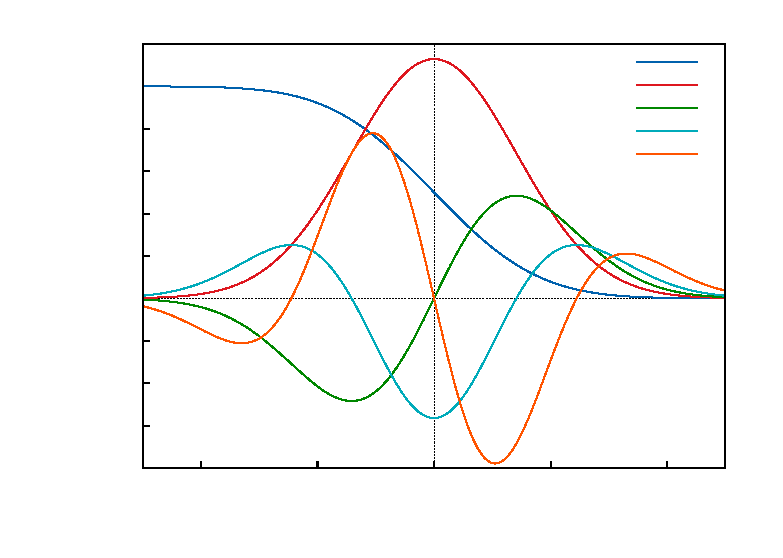
\includegraphics{./figures/gmf_tail}}%
    \gplfronttext
  \end{picture}%
\endgroup
}}\hfill
  \subfigure[$\HS=\HSC=\minfu$]{\scalebox{0.5}{% GNUPLOT: LaTeX picture with Postscript
\begingroup
  \makeatletter
  \providecommand\color[2][]{%
    \GenericError{(gnuplot) \space\space\space\@spaces}{%
      Package color not loaded in conjunction with
      terminal option `colourtext'%
    }{See the gnuplot documentation for explanation.%
    }{Either use 'blacktext' in gnuplot or load the package
      color.sty in LaTeX.}%
    \renewcommand\color[2][]{}%
  }%
  \providecommand\includegraphics[2][]{%
    \GenericError{(gnuplot) \space\space\space\@spaces}{%
      Package graphicx or graphics not loaded%
    }{See the gnuplot documentation for explanation.%
    }{The gnuplot epslatex terminal needs graphicx.sty or graphics.sty.}%
    \renewcommand\includegraphics[2][]{}%
  }%
  \providecommand\rotatebox[2]{#2}%
  \@ifundefined{ifGPcolor}{%
    \newif\ifGPcolor
    \GPcolorfalse
  }{}%
  \@ifundefined{ifGPblacktext}{%
    \newif\ifGPblacktext
    \GPblacktexttrue
  }{}%
  % define a \g@addto@macro without @ in the name:
  \let\gplgaddtomacro\g@addto@macro
  % define empty templates for all commands taking text:
  \gdef\gplbacktext{}%
  \gdef\gplfronttext{}%
  \makeatother
  \ifGPblacktext
    % no textcolor at all
    \def\colorrgb#1{}%
    \def\colorgray#1{}%
  \else
    % gray or color?
    \ifGPcolor
      \def\colorrgb#1{\color[rgb]{#1}}%
      \def\colorgray#1{\color[gray]{#1}}%
      \expandafter\def\csname LTw\endcsname{\color{white}}%
      \expandafter\def\csname LTb\endcsname{\color{black}}%
      \expandafter\def\csname LTa\endcsname{\color{black}}%
      \expandafter\def\csname LT0\endcsname{\color[rgb]{1,0,0}}%
      \expandafter\def\csname LT1\endcsname{\color[rgb]{0,1,0}}%
      \expandafter\def\csname LT2\endcsname{\color[rgb]{0,0,1}}%
      \expandafter\def\csname LT3\endcsname{\color[rgb]{1,0,1}}%
      \expandafter\def\csname LT4\endcsname{\color[rgb]{0,1,1}}%
      \expandafter\def\csname LT5\endcsname{\color[rgb]{1,1,0}}%
      \expandafter\def\csname LT6\endcsname{\color[rgb]{0,0,0}}%
      \expandafter\def\csname LT7\endcsname{\color[rgb]{1,0.3,0}}%
      \expandafter\def\csname LT8\endcsname{\color[rgb]{0.5,0.5,0.5}}%
    \else
      % gray
      \def\colorrgb#1{\color{black}}%
      \def\colorgray#1{\color[gray]{#1}}%
      \expandafter\def\csname LTw\endcsname{\color{white}}%
      \expandafter\def\csname LTb\endcsname{\color{black}}%
      \expandafter\def\csname LTa\endcsname{\color{black}}%
      \expandafter\def\csname LT0\endcsname{\color{black}}%
      \expandafter\def\csname LT1\endcsname{\color{black}}%
      \expandafter\def\csname LT2\endcsname{\color{black}}%
      \expandafter\def\csname LT3\endcsname{\color{black}}%
      \expandafter\def\csname LT4\endcsname{\color{black}}%
      \expandafter\def\csname LT5\endcsname{\color{black}}%
      \expandafter\def\csname LT6\endcsname{\color{black}}%
      \expandafter\def\csname LT7\endcsname{\color{black}}%
      \expandafter\def\csname LT8\endcsname{\color{black}}%
    \fi
  \fi
  \setlength{\unitlength}{0.0500bp}%
  \begin{picture}(7200.00,5040.00)%
    \gplgaddtomacro\gplbacktext{%
      \csname LTb\endcsname%
      \put(1078,704){\makebox(0,0)[r]{\strut{}-0.2}}%
      \put(1078,1111){\makebox(0,0)[r]{\strut{}-0.15}}%
      \put(1078,1518){\makebox(0,0)[r]{\strut{}-0.1}}%
      \put(1078,1925){\makebox(0,0)[r]{\strut{}-0.05}}%
      \put(1078,2332){\makebox(0,0)[r]{\strut{} 0}}%
      \put(1078,2740){\makebox(0,0)[r]{\strut{} 0.05}}%
      \put(1078,3147){\makebox(0,0)[r]{\strut{} 0.1}}%
      \put(1078,3554){\makebox(0,0)[r]{\strut{} 0.15}}%
      \put(1078,3961){\makebox(0,0)[r]{\strut{} 0.2}}%
      \put(1078,4368){\makebox(0,0)[r]{\strut{} 0.25}}%
      \put(1078,4775){\makebox(0,0)[r]{\strut{} 0.3}}%
      \put(1769,484){\makebox(0,0){\strut{}-4}}%
      \put(2888,484){\makebox(0,0){\strut{}-2}}%
      \put(4007,484){\makebox(0,0){\strut{} 0}}%
      \put(5125,484){\makebox(0,0){\strut{} 2}}%
      \put(6244,484){\makebox(0,0){\strut{} 4}}%
      \csname LTb\endcsname%
      \put(176,2739){\rotatebox{90}{\makebox(0,0){\strut{}$\GMFa_j(\HSC)$}}}%
      \put(4006,154){\makebox(0,0){\strut{}$\lset$}}%
    }%
    \gplgaddtomacro\gplfronttext{%
      \csname LTb\endcsname%
      \put(2530,4602){\makebox(0,0)[r]{\strut{}$j=0$ ($\bullet/4$)}}%
      \csname LTb\endcsname%
      \put(2530,4382){\makebox(0,0)[r]{\strut{}$j=1$}}%
      \csname LTb\endcsname%
      \put(2530,4162){\makebox(0,0)[r]{\strut{}$j=2$}}%
      \csname LTb\endcsname%
      \put(2530,3942){\makebox(0,0)[r]{\strut{}$j=3$}}%
      \csname LTb\endcsname%
      \put(2530,3722){\makebox(0,0)[r]{\strut{}$j=4$}}%
    }%
    \gplbacktext
    \put(0,0){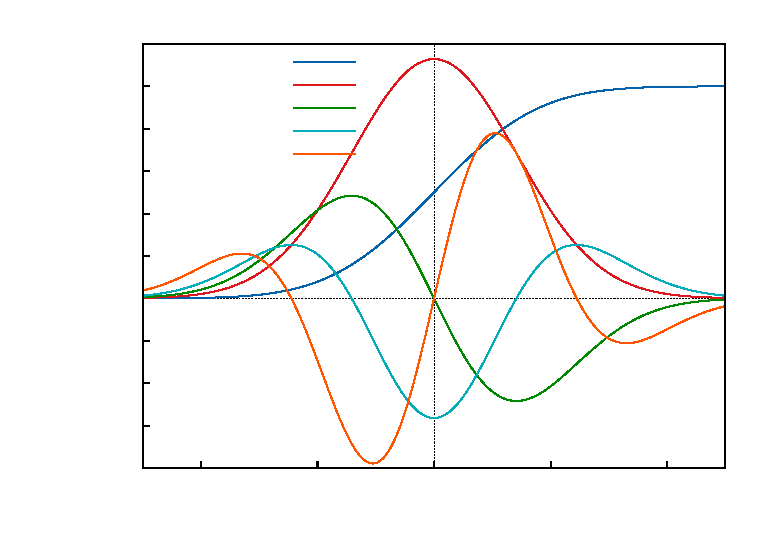
\includegraphics{./figures/gmf_cumulative}}%
    \gplfronttext
  \end{picture}%
\endgroup
}}\hspace*{\fill}
  \caption{First 4 GMF for $\std^2=2$}
\end{figure}
\item Derivatives:
\begin{equation}
  \forall j, \ \ \frac{\text{d}\GMFa_j}{\text{d}\lset}(\HSC)=\frac{\text{d}^{j+1}\CDP(\lset)}{\text{d}\lset^{j+1}}=\GMFa_{j+1}(\HSC)
\end{equation}
\end{itemize}

\subsubsection{Application to: $k\in\NZ$ and $\HS = \Rk \backslash \mathcal{B}_{\Rk}\left(0,\lset\right)$}
Simplification $\mean=0$ gives Gaussian measure:
\begin{equation}
    \gamma_k(\HS) = \frac{1}{\std^k(2\pi)^{k/2}} \int_{\HS} \ e^{-\|\x\|^2/2\std^2} d\x
\end{equation}
Spherical coordinates in $\Rk$:
\begin{equation}
  \left\{
  \begin{array}{lcl}
    \|\x\|    & = & r \\
    x_1     & = & r \cos(\theta_1) \\
    x_2     & = & r \sin(\theta_1) \cos(\theta_2) \\
    x_2     & = & r \sin(\theta_1) \sin(\theta_2) \cos(\theta_3) \\
    \vdots    & & \\
    x_{k-1} & = & r \sin(\theta_1) \sin(\theta_2) \cdots \sin(\theta_{k-2}) \cos(\theta_{k-1}) \\
    x_k     & = & r \sin(\theta_1) \sin(\theta_2) \cdots \sin(\theta_{k-2}) \sin(\theta_{k-1})
  \end{array}
  \right.
\end{equation}
Volume element in $\Rk$:
\begin{subequations}
  \begin{align*}
    dV & = \left| \text{det}\frac{\partial x_i}{\partial (r,\theta_j)} \right| dr d\theta_1\cdots d\theta_{k-1} \\
       & = r^{k-1}\sin^{k-2}(\theta_1) \sin^{k-3}(\theta_2) \cdots \sin(\theta_{k-2}) dr d\theta_1\cdots d\theta_{k-1}
  \end{align*}
\end{subequations}
Gaussian volume using $(r,\{\theta_i\})$:
\begin{equation}
  \begin{aligned}
    \gamma_k(\Rk \backslash \mathcal{B}_{\Rk}(0,\lset)) & = \frac{1}{\std^k(2\pi)^{k/2}} \int_{r=\lset}^\infty \ r^{k-1} e^{-r^2/2\std^2} dr \\
                                       & \times \underbrace{\int_0^\pi \sin^{k-2}(\theta_1)d\theta_1\int_0^{2\pi}\sin^{k-3}(\theta_2)d\theta_2 \cdots \int_0^{2\pi}d\theta_{k-1}}_{2\pi^{k/2}/\Gamma(k/2) \ \ (k-1\text{-dimensional volume of unit sphere})} \\ \\
                                       & = \frac{1}{\std^k2^{k/2-1}\Gamma(k/2)} \int_{r=\lset}^\infty \ r^{k-1} e^{-r^2/2\std^2} dr
  \end{aligned}
\end{equation}
Tube expansion for $\HS=\Rk \backslash \mathcal{B}_{\Rk}(0,\lset)$:
\begin{equation}
  \GaussMeas^k(\tube(\Rk \backslash \mathcal{B}_{\Rk}\left(0,\lset\right),\ray))=\GaussMeas^k(\Rk \backslash \mathcal{B}_{\Rk}\left(0,\lset-\ray\right))=\sum_{j=0}^{\infty} \frac{(-\ray)^j}{j!} \frac{\text{d}^j \gamma_k(\Rk \backslash \mathcal{B}_{\Rk}(0,\lset))}{\text{d} \lset^j}
\end{equation}
Simplification of $\gamma_k(\Rk \backslash \mathcal{B}_{\Rk}(0,\lset))$ with variable substitution:
\begin{equation}
  \left\{
  \begin{array}{lll}
    t = r^2/2\std^2 &\rightarrow& r = \sqrt{2t}\std \\
    dt = rdr/\std^2 &\rightarrow& dr= \sqrt{1/2t}\std dt
  \end{array}
  \right.
\end{equation}
\begin{equation}
  \begin{aligned}
    \gamma_k(\Rk \backslash \mathcal{B}_{\Rk}(0,\lset)) & = \frac{1}{\std^k\Gamma(k/2)2^{k/2-1}} \int_{t=\lset^2/2\std^2}^\infty \ (\sqrt{2t}\std)^{k-1} e^{-t} \frac{\std}{\sqrt{2t}} dt\\
                  & = \frac{1}{\Gamma(k/2)} \int_{t=\lset^2/2\std^2}^\infty \ t^{k/2-1} e^{-t} dt\\
                  & = \overline{\Gamma}(k/2,\lset^2/2\std^2)
  \end{aligned}
\end{equation}

\subsubsection{Application to: $k\in\NZ$ for various $\HS$}
\begin{equation}
  \begin{array}{lll}
    \gamma_k(\mathcal{B}_{\Rk}(0,\lset))              &=& \overline{\gamma}(k/2,\lset^2/2\std^2) \\
    \gamma_k(\Rk\backslash\mathcal{B}_{\Rk}(0,\lset)) &=& \overline{\Gamma}(k/2,\lset^2/2\std^2) \\
    \gamma_k(\mathcal{B}_{\Rk}(0,\lset_1)\cup(\Rk\backslash\mathcal{B}_{\Rk}(0,\lset_2)))) &=& \overline{\gamma}(k/2,\lset_1^2/2\std^2) + \overline{\Gamma}(k/2,\lset_2^2/2\std^2) \\
    \gamma_k(\Rk\backslash(\mathcal{B}_{\Rk}(0,\lset_1)\cup(\Rk\backslash\mathcal{B}_{\Rk}(0,\lset_2))))) &=& 1-\overline{\gamma}(k/2,\lset_1^2/2\std^2) - \overline{\Gamma}(k/2,\lset_2^2/2\std^2)
  \end{array}
\end{equation}


\subsection{GMFs for Gaussian related Random Fields}
\begin{equation}
  \GRRF : \Univ\times\RN \overset{\vGRF}{\rightarrow} \Rk \overset{\rfunc}{\rightarrow} \RR
\end{equation}
\begin{equation}
    \Proba\left\{\GRRF\in\HS\right\} = \Proba\left\{\rfunc(\GRF)\in\HS\right\} = \Proba\left\{\GRF\in\irfunc(\HS)\right\} = \GaussMeas^k(\irfunc(\HS))
\end{equation}

\subsubsection{Log-normal distribution}
\begin{equation}
  k=1, \ \ \rfunc:\RR\mapsto\RR=\exp \ \ \text{and} \ \ \irfunc=\ln
\end{equation}
\begin{equation}
  \left|
  \begin{array}{lcl}
    \mean & = &\ln(\meanln) - \frac{1}{2}\ln(1+\stdln^2/\meanln^2) \\
    \std^2 & = & \ln(1+\stdln^2/\meanln^2)
  \end{array}
  \right.
\end{equation}

\begin{itemize}
\item Notations:
  \begin{subequations}
    \begin{flalign}
      & \text{Log tail hitting set:} \ \ \lnHST=\lnuinf & \\
      & \text{Log cumulative hitting set:} \ \ \lnHSC = \minflnu & \\
      & \text{Variable substitution:} \ \ \lnclset \leftarrow \frac{\ln(\lset)-\mean}{\std} &
    \end{flalign}
  \end{subequations}
\item For $\HS=\HST=\uinf \ \ \rightarrow \ \ \irfunc(\HS) = \lnHST = \lnuinf$
\begin{equation}
  \left|
  \begin{array}{l}
    \GMFa_0(\lnHST) = \frac{1}{2}\left(1-\erf\left(\frac{\lnclset}{\sqrt{2}}\right)\right) \\ \\
    \GMFa_1(\lnHST) = \frac{1}{\std  \sqrt{2\pi}}\ e^{-\lnclset^2/2} \\ \\
    \GMFa_2(\lnHST) = \frac{1}{\std^2\sqrt{2\pi}}\ \lnclset \ e^{-\lnclset^2/2} \\ \\
    \GMFa_3(\lnHST) = \frac{1}{\std^3\sqrt{2\pi}}\ \left(\lnclset^2-1\right) \ e^{-\lnclset^2/2} \\ \\
    \GMFa_4(\lnHST) = \frac{1}{\std^4\sqrt{2\pi}}\ \left(\lnclset^3-3\lnclset\right) \ e^{-\lnclset^2/2} \\ \\
    \dots
  \end{array}
  \right.
\end{equation}
Derivatives:
\begin{equation}
  \left|
  \begin{array}{l}
    \text{Help:} \ \ \left(e^{-(\ln(x)-\mean)^2/2\std^2}\right)' = -\frac{1}{\std^2} \frac{\ln(x)-\mean}{x}\ e^{-(\ln(x)-\mean)^2/2\std^2} \\ \\
    \frac{\text{d} \GMFa_0(\lnHST)}{\text{d}\lset} = \frac{-1}{\std\sqrt{2\pi}} \frac{1}{\lset}\ e^{-(\ln(\lset)-\mean)^2/2\std^2} \\ \\
    \frac{\text{d} \GMFa_1(\lnHST)}{\text{d}\lset} = \frac{-1}{\std^2\sqrt{2\pi}} \frac{1}{\lset}\frac{\ln(\lset)-\mean}{\std}\ e^{-(\ln(\lset)-\mean)^2/2\std^2} \\ \\
    \frac{\text{d} \GMFa_2(\lnHST)}{\text{d}\lset} = \frac{-1}{\std^3\sqrt{2\pi}} \frac{1}{\lset}\left[ \frac{(\ln(\lset)-\mean)^2}{\std^2} - 1 \right]\ e^{-(\ln(\lset)-\mean)^2/2\std^2} \\ \\
    \frac{\text{d} \GMFa_3(\lnHST)}{\text{d}\lset} = \frac{-1}{\std^4\sqrt{2\pi}} \frac{1}{\lset}\left[ \frac{(\ln(\lset)-\mean)^3}{\std^3} - 3\frac{(\ln(\lset)-\mean)}{\std} \right]\ e^{-(\ln(\lset)-\mean)^2/2\std^2} \\ \\
    \dots \\ \\
    \text{Guess would be:} \ \ \forall j\ge0, \\
    \frac{\text{d} \GMFa_j(\lnHST)}{\text{d}\lset} = \frac{-1}{\std^{j+1}\sqrt{2\pi}}\frac{1}{\lset}\Hermite_{j}(\lnclset)\ e^{-\lnclset^2/2}
  \end{array}
  \right.
\end{equation}

\item For $\HS=\zu \ \ \rightarrow \ \ \irfunc(\HS) = \lnHSC = \minflnu$
\begin{equation}
  \left|
  \begin{array}{l}
    \GMFa_0(\lnHSC) = \frac{1}{2}\left(1+\erf\left(\frac{\lnclset}{\sqrt{2}}\right)\right) \\ \\
    \GMFa_1(\lnHSC) = \frac{1}{\std  \sqrt{2\pi}}\ e^{-\lnclset^2/2} \\ \\
    \GMFa_2(\lnHSC) = \frac{-1}{\std^2\sqrt{2\pi}}\ \lnclset \ e^{-\lnclset^2/2} \\ \\
    \GMFa_3(\lnHSC) = \frac{1}{\std^3\sqrt{2\pi}}\ \left(\lnclset^2-1\right) \ e^{-\lnclset^2/2} \\ \\
    \GMFa_4(\lnHSC) = \frac{-1}{\std^4\sqrt{2\pi}}\ \left(\lnclset^3-3\lnclset\right) \ e^{-\lnclset^2/2} \\ \\
    \dots
  \end{array}
  \right.
\end{equation}
Derivatives:
\begin{equation}
  \left|
  \begin{array}{l}
    \text{Guess would be:} \ \ \forall j\ge0, \\
    \frac{\text{d} \GMFa_j(\lnHSC)}{\text{d}\lset} = \frac{(-1)^{j}}{\std^{j+1}\sqrt{2\pi}}\frac{1}{\lset}\Hermite_{j}(\lnclset)\ e^{-\lnclset^2/2}
  \end{array}
  \right.
\end{equation}
\end{itemize}

\subsubsection{$\chi^2_k$ distribution}
\begin{equation}
  k\in\NZ, \ \ \rfunc:\Rk\mapsto\RR=\|\bullet\|_2
\end{equation}
Identification with tail hitting set:
\begin{equation}
  \HSTchik=\irfunc(\uinf)=\mathcal{B}_{\Rk}\left(0,\sqrt{\lset}\right)
\end{equation}

\begin{itemize}
\item For $j=0$:
\begin{equation}
  \GMFk_0(\HSTchik)=\overline{\Gamma}(k/2,\lset/2\std^2)
\end{equation}
\item For $j=1$:
\begin{equation}
  \GMFk_1(\HSTchik)=-\frac{\text{d}\overline{\Gamma}(k/2,\lset/2\std^2)}{\text{d}\lset}=\left(\frac{\lset}{2\std^2}\right)^{k/2-1}e^{-\lset/2\std^2}
\end{equation}
\item For $j>1$:
  \begin{equation}
    \begin{aligned}
      \GMFk_j(\HSTchik)&=(-1)^j\frac{\text{d}^j\overline{\Gamma}(k/2,\lset/2\std^2)}{\text{d}\lset^j}\\
                       &=\frac{1}{(2\std^2)^{2j-2}}\prod_{l=1}^{j-1}\left(\frac{k}{2}-l\right)\left(\frac{\lset}{2\std^2}\right)^{k/2-j}e^{-\lset/2\std^2}
    \end{aligned}
  \end{equation}

\item First values:
  \begin{equation}
    \left\{
    \begin{aligned}
      &\GMFk_0(\HSTchik) = \int_{\frac{\lset}{2\std^2}}^\infty t^{k/2-1}e^{-t} dt\\ 
      &\GMFk_1(\HSTchik) = \left(\frac{\lset}{2\std^2}\right)^{k/2-1}e^{-\lset/2\std^2}\\
      &\GMFk_2(\HSTchik) = \frac{1}{(2\std^2)^2}\left[\frac{k}{2}-1\right] \left(\frac{\lset}{2\std^2}\right)^{k/2-2}e^{-\lset/2\std^2}\\
      &\GMFk_3(\HSTchik) = \frac{1}{(2\std^2)^4}\left[\left(\frac{k}{2}-1\right)\left(\frac{k}{2}-2\right)\right] \left(\frac{\lset}{2\std^2}\right)^{k/2-3}e^{-\lset/2\std^2}\\
      &\GMFk_4(\HSTchik) = \frac{1}{(2\std^2)^6}\left[\left(\frac{k}{2}-1\right)\left(\frac{k}{2}-2\right)\left(\frac{k}{2}-3\right)\right] \left(\frac{\lset}{2\std^2}\right)^{k/2-4}e^{-\lset/2\std^2}\\
      &\dots \\
    \end{aligned}
    \right.
  \end{equation}
\end{itemize}

\newpage
\section{Expectation Formula}
\subsection{General case}
\begin{equation}
  \Expec\left\{\ \LKC_j(\ES) \ \right\} = \sum_{i=0}^{N-j} \left[ \begin{array}{c}i+j\\i\end{array}\right]\left(\frac{\SpecMom}{2\pi}\right)^{i/2}\LKC_{i+j}(\MRF)\GMFk_i(\irfunc(\HS))
\end{equation}
Notations:
  \begin{subequations}
    \begin{flalign}
      & \text{LKC of $\MRF$:} \ \ \LKC_j(\MRF) = \LKC_j^\MRF & \\
      & \text{LKC of $\ES$:} \ \ \LKC_j(\ES) = \LKC_j^\ES & \\
      & \text{GMF of $\irfunc(\HS)$:} \ \  \GMFk_j(\irfunc(\HS)) = \GMFk_j
    \end{flalign}
  \end{subequations}
\subsection{One dimension}
\begin{subequations}
\begin{align}
  &\Expec\left\{\LKC_0^\ES\right\} = \left(\frac{\SpecMom}{2\pi}\right)^{1/2}\LKC_1^\MRF\GMFk_1 + \LKC_0^\MRF\GMFk_0\\
  &\Expec\left\{\LKC_1^\ES\right\} = \LKC_1^\MRF\GMFk_0
\end{align}
\end{subequations}


\begin{figure}[!h]
  \centering
  \hspace*{\fill}
  \subfigure[Euler Characteristic]{\scalebox{0.5}{% GNUPLOT: LaTeX picture with Postscript
\begingroup
  \makeatletter
  \providecommand\color[2][]{%
    \GenericError{(gnuplot) \space\space\space\@spaces}{%
      Package color not loaded in conjunction with
      terminal option `colourtext'%
    }{See the gnuplot documentation for explanation.%
    }{Either use 'blacktext' in gnuplot or load the package
      color.sty in LaTeX.}%
    \renewcommand\color[2][]{}%
  }%
  \providecommand\includegraphics[2][]{%
    \GenericError{(gnuplot) \space\space\space\@spaces}{%
      Package graphicx or graphics not loaded%
    }{See the gnuplot documentation for explanation.%
    }{The gnuplot epslatex terminal needs graphicx.sty or graphics.sty.}%
    \renewcommand\includegraphics[2][]{}%
  }%
  \providecommand\rotatebox[2]{#2}%
  \@ifundefined{ifGPcolor}{%
    \newif\ifGPcolor
    \GPcolorfalse
  }{}%
  \@ifundefined{ifGPblacktext}{%
    \newif\ifGPblacktext
    \GPblacktexttrue
  }{}%
  % define a \g@addto@macro without @ in the name:
  \let\gplgaddtomacro\g@addto@macro
  % define empty templates for all commands taking text:
  \gdef\gplbacktext{}%
  \gdef\gplfronttext{}%
  \makeatother
  \ifGPblacktext
    % no textcolor at all
    \def\colorrgb#1{}%
    \def\colorgray#1{}%
  \else
    % gray or color?
    \ifGPcolor
      \def\colorrgb#1{\color[rgb]{#1}}%
      \def\colorgray#1{\color[gray]{#1}}%
      \expandafter\def\csname LTw\endcsname{\color{white}}%
      \expandafter\def\csname LTb\endcsname{\color{black}}%
      \expandafter\def\csname LTa\endcsname{\color{black}}%
      \expandafter\def\csname LT0\endcsname{\color[rgb]{1,0,0}}%
      \expandafter\def\csname LT1\endcsname{\color[rgb]{0,1,0}}%
      \expandafter\def\csname LT2\endcsname{\color[rgb]{0,0,1}}%
      \expandafter\def\csname LT3\endcsname{\color[rgb]{1,0,1}}%
      \expandafter\def\csname LT4\endcsname{\color[rgb]{0,1,1}}%
      \expandafter\def\csname LT5\endcsname{\color[rgb]{1,1,0}}%
      \expandafter\def\csname LT6\endcsname{\color[rgb]{0,0,0}}%
      \expandafter\def\csname LT7\endcsname{\color[rgb]{1,0.3,0}}%
      \expandafter\def\csname LT8\endcsname{\color[rgb]{0.5,0.5,0.5}}%
    \else
      % gray
      \def\colorrgb#1{\color{black}}%
      \def\colorgray#1{\color[gray]{#1}}%
      \expandafter\def\csname LTw\endcsname{\color{white}}%
      \expandafter\def\csname LTb\endcsname{\color{black}}%
      \expandafter\def\csname LTa\endcsname{\color{black}}%
      \expandafter\def\csname LT0\endcsname{\color{black}}%
      \expandafter\def\csname LT1\endcsname{\color{black}}%
      \expandafter\def\csname LT2\endcsname{\color{black}}%
      \expandafter\def\csname LT3\endcsname{\color{black}}%
      \expandafter\def\csname LT4\endcsname{\color{black}}%
      \expandafter\def\csname LT5\endcsname{\color{black}}%
      \expandafter\def\csname LT6\endcsname{\color{black}}%
      \expandafter\def\csname LT7\endcsname{\color{black}}%
      \expandafter\def\csname LT8\endcsname{\color{black}}%
    \fi
  \fi
  \setlength{\unitlength}{0.0500bp}%
  \begin{picture}(7200.00,5040.00)%
    \gplgaddtomacro\gplbacktext{%
      \csname LTb\endcsname%
      \put(946,704){\makebox(0,0)[r]{\strut{} 0}}%
      \put(946,1213){\makebox(0,0)[r]{\strut{} 0.2}}%
      \put(946,1722){\makebox(0,0)[r]{\strut{} 0.4}}%
      \put(946,2231){\makebox(0,0)[r]{\strut{} 0.6}}%
      \put(946,2740){\makebox(0,0)[r]{\strut{} 0.8}}%
      \put(946,3248){\makebox(0,0)[r]{\strut{} 1}}%
      \put(946,3757){\makebox(0,0)[r]{\strut{} 1.2}}%
      \put(946,4266){\makebox(0,0)[r]{\strut{} 1.4}}%
      \put(946,4775){\makebox(0,0)[r]{\strut{} 1.6}}%
      \put(1651,484){\makebox(0,0){\strut{}-4}}%
      \put(2796,484){\makebox(0,0){\strut{}-2}}%
      \put(3941,484){\makebox(0,0){\strut{} 0}}%
      \put(5086,484){\makebox(0,0){\strut{} 2}}%
      \put(6231,484){\makebox(0,0){\strut{} 4}}%
      \csname LTb\endcsname%
      \put(176,2739){\rotatebox{90}{\makebox(0,0){\strut{}Euleru characteristic}}}%
      \put(3940,154){\makebox(0,0){\strut{}$\lset$}}%
    }%
    \gplgaddtomacro\gplfronttext{%
      \csname LTb\endcsname%
      \put(5816,4602){\makebox(0,0)[r]{\strut{}$\Lc=25$}}%
      \csname LTb\endcsname%
      \put(5816,4382){\makebox(0,0)[r]{\strut{}$\Lc=50$}}%
      \csname LTb\endcsname%
      \put(5816,4162){\makebox(0,0)[r]{\strut{}$\Lc=100$}}%
      \csname LTb\endcsname%
      \put(5816,3942){\makebox(0,0)[r]{\strut{}$\Lc=500$}}%
      \csname LTb\endcsname%
      \put(5816,3722){\makebox(0,0)[r]{\strut{}$\Lc=1000$}}%
    }%
    \gplbacktext
    \put(0,0){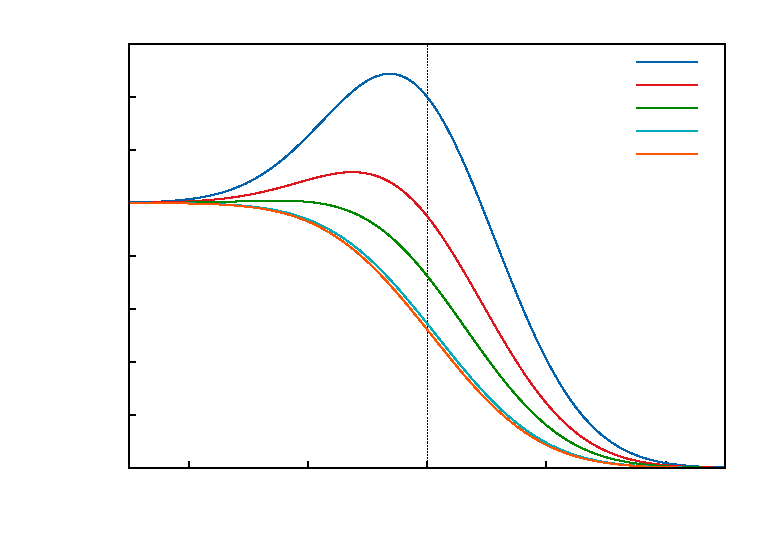
\includegraphics{./figures/elkc_1D_LKC0}}%
    \gplfronttext
  \end{picture}%
\endgroup
}}\hfill
  \subfigure[Length]{\scalebox{0.5}{% GNUPLOT: LaTeX picture with Postscript
\begingroup
  \makeatletter
  \providecommand\color[2][]{%
    \GenericError{(gnuplot) \space\space\space\@spaces}{%
      Package color not loaded in conjunction with
      terminal option `colourtext'%
    }{See the gnuplot documentation for explanation.%
    }{Either use 'blacktext' in gnuplot or load the package
      color.sty in LaTeX.}%
    \renewcommand\color[2][]{}%
  }%
  \providecommand\includegraphics[2][]{%
    \GenericError{(gnuplot) \space\space\space\@spaces}{%
      Package graphicx or graphics not loaded%
    }{See the gnuplot documentation for explanation.%
    }{The gnuplot epslatex terminal needs graphicx.sty or graphics.sty.}%
    \renewcommand\includegraphics[2][]{}%
  }%
  \providecommand\rotatebox[2]{#2}%
  \@ifundefined{ifGPcolor}{%
    \newif\ifGPcolor
    \GPcolorfalse
  }{}%
  \@ifundefined{ifGPblacktext}{%
    \newif\ifGPblacktext
    \GPblacktexttrue
  }{}%
  % define a \g@addto@macro without @ in the name:
  \let\gplgaddtomacro\g@addto@macro
  % define empty templates for all commands taking text:
  \gdef\gplbacktext{}%
  \gdef\gplfronttext{}%
  \makeatother
  \ifGPblacktext
    % no textcolor at all
    \def\colorrgb#1{}%
    \def\colorgray#1{}%
  \else
    % gray or color?
    \ifGPcolor
      \def\colorrgb#1{\color[rgb]{#1}}%
      \def\colorgray#1{\color[gray]{#1}}%
      \expandafter\def\csname LTw\endcsname{\color{white}}%
      \expandafter\def\csname LTb\endcsname{\color{black}}%
      \expandafter\def\csname LTa\endcsname{\color{black}}%
      \expandafter\def\csname LT0\endcsname{\color[rgb]{1,0,0}}%
      \expandafter\def\csname LT1\endcsname{\color[rgb]{0,1,0}}%
      \expandafter\def\csname LT2\endcsname{\color[rgb]{0,0,1}}%
      \expandafter\def\csname LT3\endcsname{\color[rgb]{1,0,1}}%
      \expandafter\def\csname LT4\endcsname{\color[rgb]{0,1,1}}%
      \expandafter\def\csname LT5\endcsname{\color[rgb]{1,1,0}}%
      \expandafter\def\csname LT6\endcsname{\color[rgb]{0,0,0}}%
      \expandafter\def\csname LT7\endcsname{\color[rgb]{1,0.3,0}}%
      \expandafter\def\csname LT8\endcsname{\color[rgb]{0.5,0.5,0.5}}%
    \else
      % gray
      \def\colorrgb#1{\color{black}}%
      \def\colorgray#1{\color[gray]{#1}}%
      \expandafter\def\csname LTw\endcsname{\color{white}}%
      \expandafter\def\csname LTb\endcsname{\color{black}}%
      \expandafter\def\csname LTa\endcsname{\color{black}}%
      \expandafter\def\csname LT0\endcsname{\color{black}}%
      \expandafter\def\csname LT1\endcsname{\color{black}}%
      \expandafter\def\csname LT2\endcsname{\color{black}}%
      \expandafter\def\csname LT3\endcsname{\color{black}}%
      \expandafter\def\csname LT4\endcsname{\color{black}}%
      \expandafter\def\csname LT5\endcsname{\color{black}}%
      \expandafter\def\csname LT6\endcsname{\color{black}}%
      \expandafter\def\csname LT7\endcsname{\color{black}}%
      \expandafter\def\csname LT8\endcsname{\color{black}}%
    \fi
  \fi
  \setlength{\unitlength}{0.0500bp}%
  \begin{picture}(7200.00,5040.00)%
    \gplgaddtomacro\gplbacktext{%
      \csname LTb\endcsname%
      \put(946,704){\makebox(0,0)[r]{\strut{} 0}}%
      \put(946,1111){\makebox(0,0)[r]{\strut{} 10}}%
      \put(946,1518){\makebox(0,0)[r]{\strut{} 20}}%
      \put(946,1925){\makebox(0,0)[r]{\strut{} 30}}%
      \put(946,2332){\makebox(0,0)[r]{\strut{} 40}}%
      \put(946,2740){\makebox(0,0)[r]{\strut{} 50}}%
      \put(946,3147){\makebox(0,0)[r]{\strut{} 60}}%
      \put(946,3554){\makebox(0,0)[r]{\strut{} 70}}%
      \put(946,3961){\makebox(0,0)[r]{\strut{} 80}}%
      \put(946,4368){\makebox(0,0)[r]{\strut{} 90}}%
      \put(946,4775){\makebox(0,0)[r]{\strut{} 100}}%
      \put(1651,484){\makebox(0,0){\strut{}-4}}%
      \put(2796,484){\makebox(0,0){\strut{}-2}}%
      \put(3941,484){\makebox(0,0){\strut{} 0}}%
      \put(5086,484){\makebox(0,0){\strut{} 2}}%
      \put(6231,484){\makebox(0,0){\strut{} 4}}%
      \csname LTb\endcsname%
      \put(176,2739){\rotatebox{90}{\makebox(0,0){\strut{}Length}}}%
      \put(3940,154){\makebox(0,0){\strut{}$\lset$}}%
    }%
    \gplgaddtomacro\gplfronttext{%
    }%
    \gplbacktext
    \put(0,0){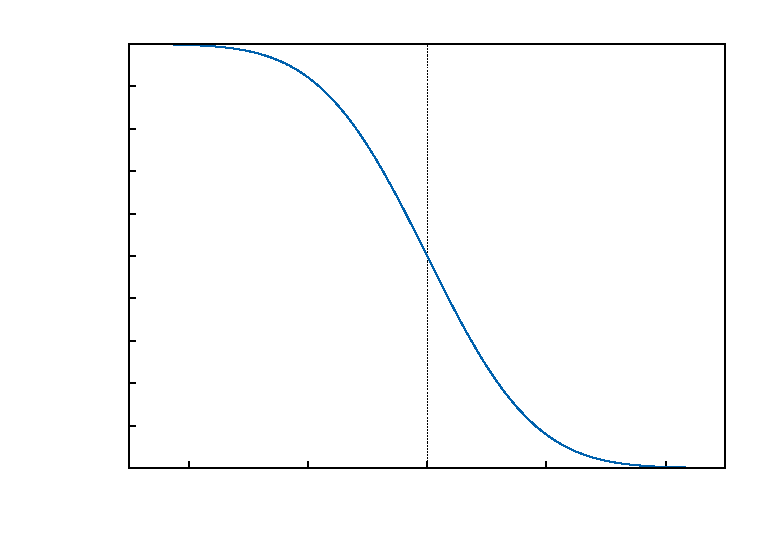
\includegraphics{./figures/elkc_1D_LKC1}}%
    \gplfronttext
  \end{picture}%
\endgroup
}}\hspace*{\fill}
  \caption{Expectation of LKC for $\Msize=100$, $\std^2=2$ and $\HS=\uinf$ in 1D.}
\end{figure}

\begin{figure}[!h]
  \centering
  \hspace*{\fill}
  \subfigure{\scalebox{0.5}{% GNUPLOT: LaTeX picture with Postscript
\begingroup
  \makeatletter
  \providecommand\color[2][]{%
    \GenericError{(gnuplot) \space\space\space\@spaces}{%
      Package color not loaded in conjunction with
      terminal option `colourtext'%
    }{See the gnuplot documentation for explanation.%
    }{Either use 'blacktext' in gnuplot or load the package
      color.sty in LaTeX.}%
    \renewcommand\color[2][]{}%
  }%
  \providecommand\includegraphics[2][]{%
    \GenericError{(gnuplot) \space\space\space\@spaces}{%
      Package graphicx or graphics not loaded%
    }{See the gnuplot documentation for explanation.%
    }{The gnuplot epslatex terminal needs graphicx.sty or graphics.sty.}%
    \renewcommand\includegraphics[2][]{}%
  }%
  \providecommand\rotatebox[2]{#2}%
  \@ifundefined{ifGPcolor}{%
    \newif\ifGPcolor
    \GPcolorfalse
  }{}%
  \@ifundefined{ifGPblacktext}{%
    \newif\ifGPblacktext
    \GPblacktexttrue
  }{}%
  % define a \g@addto@macro without @ in the name:
  \let\gplgaddtomacro\g@addto@macro
  % define empty templates for all commands taking text:
  \gdef\gplbacktext{}%
  \gdef\gplfronttext{}%
  \makeatother
  \ifGPblacktext
    % no textcolor at all
    \def\colorrgb#1{}%
    \def\colorgray#1{}%
  \else
    % gray or color?
    \ifGPcolor
      \def\colorrgb#1{\color[rgb]{#1}}%
      \def\colorgray#1{\color[gray]{#1}}%
      \expandafter\def\csname LTw\endcsname{\color{white}}%
      \expandafter\def\csname LTb\endcsname{\color{black}}%
      \expandafter\def\csname LTa\endcsname{\color{black}}%
      \expandafter\def\csname LT0\endcsname{\color[rgb]{1,0,0}}%
      \expandafter\def\csname LT1\endcsname{\color[rgb]{0,1,0}}%
      \expandafter\def\csname LT2\endcsname{\color[rgb]{0,0,1}}%
      \expandafter\def\csname LT3\endcsname{\color[rgb]{1,0,1}}%
      \expandafter\def\csname LT4\endcsname{\color[rgb]{0,1,1}}%
      \expandafter\def\csname LT5\endcsname{\color[rgb]{1,1,0}}%
      \expandafter\def\csname LT6\endcsname{\color[rgb]{0,0,0}}%
      \expandafter\def\csname LT7\endcsname{\color[rgb]{1,0.3,0}}%
      \expandafter\def\csname LT8\endcsname{\color[rgb]{0.5,0.5,0.5}}%
    \else
      % gray
      \def\colorrgb#1{\color{black}}%
      \def\colorgray#1{\color[gray]{#1}}%
      \expandafter\def\csname LTw\endcsname{\color{white}}%
      \expandafter\def\csname LTb\endcsname{\color{black}}%
      \expandafter\def\csname LTa\endcsname{\color{black}}%
      \expandafter\def\csname LT0\endcsname{\color{black}}%
      \expandafter\def\csname LT1\endcsname{\color{black}}%
      \expandafter\def\csname LT2\endcsname{\color{black}}%
      \expandafter\def\csname LT3\endcsname{\color{black}}%
      \expandafter\def\csname LT4\endcsname{\color{black}}%
      \expandafter\def\csname LT5\endcsname{\color{black}}%
      \expandafter\def\csname LT6\endcsname{\color{black}}%
      \expandafter\def\csname LT7\endcsname{\color{black}}%
      \expandafter\def\csname LT8\endcsname{\color{black}}%
    \fi
  \fi
  \setlength{\unitlength}{0.0500bp}%
  \begin{picture}(7200.00,5040.00)%
    \gplgaddtomacro\gplbacktext{%
      \csname LTb\endcsname%
      \put(814,704){\makebox(0,0)[r]{\strut{} 0}}%
      \put(814,1286){\makebox(0,0)[r]{\strut{} 5}}%
      \put(814,1867){\makebox(0,0)[r]{\strut{} 10}}%
      \put(814,2449){\makebox(0,0)[r]{\strut{} 15}}%
      \put(814,3030){\makebox(0,0)[r]{\strut{} 20}}%
      \put(814,3612){\makebox(0,0)[r]{\strut{} 25}}%
      \put(814,4193){\makebox(0,0)[r]{\strut{} 30}}%
      \put(814,4775){\makebox(0,0)[r]{\strut{} 35}}%
      \put(946,484){\makebox(0,0){\strut{} 0.01}}%
      \put(2117,484){\makebox(0,0){\strut{} 0.1}}%
      \put(3289,484){\makebox(0,0){\strut{} 1}}%
      \put(4460,484){\makebox(0,0){\strut{} 10}}%
      \put(5632,484){\makebox(0,0){\strut{} 100}}%
      \put(6803,484){\makebox(0,0){\strut{} 1000}}%
      \csname LTb\endcsname%
      \put(176,2739){\rotatebox{90}{\makebox(0,0){\strut{}Euler characteristic $\EC$}}}%
      \put(3874,154){\makebox(0,0){\strut{}$\lset$}}%
    }%
    \gplgaddtomacro\gplfronttext{%
      \csname LTb\endcsname%
      \put(5816,4602){\makebox(0,0)[r]{\strut{}Experimental}}%
      \csname LTb\endcsname%
      \put(5816,4382){\makebox(0,0)[r]{\strut{}Theoretical}}%
      \csname LTb\endcsname%
      \put(5816,4162){\makebox(0,0)[r]{\strut{}One realization}}%
    }%
    \gplbacktext
    \put(0,0){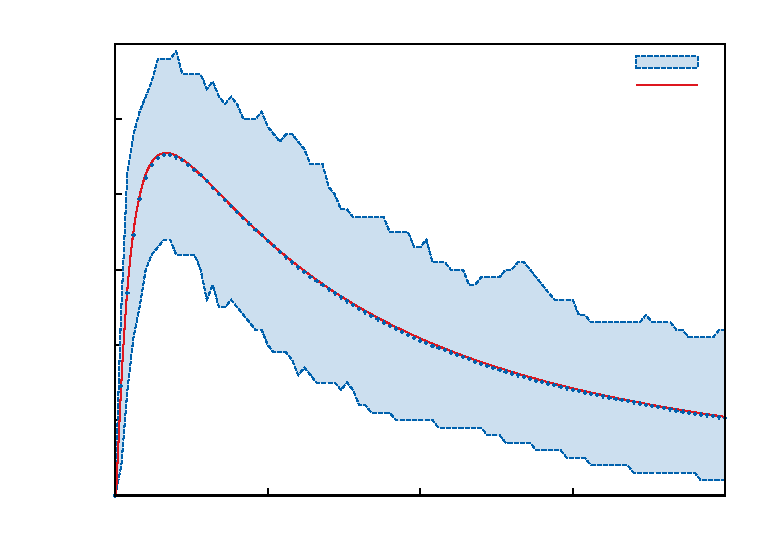
\includegraphics{./figures/elkc_exp_1D_lognormal_0}}%
    \gplfronttext
  \end{picture}%
\endgroup
}}\hfill
  \subfigure{\scalebox{0.5}{% GNUPLOT: LaTeX picture with Postscript
\begingroup
  \makeatletter
  \providecommand\color[2][]{%
    \GenericError{(gnuplot) \space\space\space\@spaces}{%
      Package color not loaded in conjunction with
      terminal option `colourtext'%
    }{See the gnuplot documentation for explanation.%
    }{Either use 'blacktext' in gnuplot or load the package
      color.sty in LaTeX.}%
    \renewcommand\color[2][]{}%
  }%
  \providecommand\includegraphics[2][]{%
    \GenericError{(gnuplot) \space\space\space\@spaces}{%
      Package graphicx or graphics not loaded%
    }{See the gnuplot documentation for explanation.%
    }{The gnuplot epslatex terminal needs graphicx.sty or graphics.sty.}%
    \renewcommand\includegraphics[2][]{}%
  }%
  \providecommand\rotatebox[2]{#2}%
  \@ifundefined{ifGPcolor}{%
    \newif\ifGPcolor
    \GPcolorfalse
  }{}%
  \@ifundefined{ifGPblacktext}{%
    \newif\ifGPblacktext
    \GPblacktexttrue
  }{}%
  % define a \g@addto@macro without @ in the name:
  \let\gplgaddtomacro\g@addto@macro
  % define empty templates for all commands taking text:
  \gdef\gplbacktext{}%
  \gdef\gplfronttext{}%
  \makeatother
  \ifGPblacktext
    % no textcolor at all
    \def\colorrgb#1{}%
    \def\colorgray#1{}%
  \else
    % gray or color?
    \ifGPcolor
      \def\colorrgb#1{\color[rgb]{#1}}%
      \def\colorgray#1{\color[gray]{#1}}%
      \expandafter\def\csname LTw\endcsname{\color{white}}%
      \expandafter\def\csname LTb\endcsname{\color{black}}%
      \expandafter\def\csname LTa\endcsname{\color{black}}%
      \expandafter\def\csname LT0\endcsname{\color[rgb]{1,0,0}}%
      \expandafter\def\csname LT1\endcsname{\color[rgb]{0,1,0}}%
      \expandafter\def\csname LT2\endcsname{\color[rgb]{0,0,1}}%
      \expandafter\def\csname LT3\endcsname{\color[rgb]{1,0,1}}%
      \expandafter\def\csname LT4\endcsname{\color[rgb]{0,1,1}}%
      \expandafter\def\csname LT5\endcsname{\color[rgb]{1,1,0}}%
      \expandafter\def\csname LT6\endcsname{\color[rgb]{0,0,0}}%
      \expandafter\def\csname LT7\endcsname{\color[rgb]{1,0.3,0}}%
      \expandafter\def\csname LT8\endcsname{\color[rgb]{0.5,0.5,0.5}}%
    \else
      % gray
      \def\colorrgb#1{\color{black}}%
      \def\colorgray#1{\color[gray]{#1}}%
      \expandafter\def\csname LTw\endcsname{\color{white}}%
      \expandafter\def\csname LTb\endcsname{\color{black}}%
      \expandafter\def\csname LTa\endcsname{\color{black}}%
      \expandafter\def\csname LT0\endcsname{\color{black}}%
      \expandafter\def\csname LT1\endcsname{\color{black}}%
      \expandafter\def\csname LT2\endcsname{\color{black}}%
      \expandafter\def\csname LT3\endcsname{\color{black}}%
      \expandafter\def\csname LT4\endcsname{\color{black}}%
      \expandafter\def\csname LT5\endcsname{\color{black}}%
      \expandafter\def\csname LT6\endcsname{\color{black}}%
      \expandafter\def\csname LT7\endcsname{\color{black}}%
      \expandafter\def\csname LT8\endcsname{\color{black}}%
    \fi
  \fi
  \setlength{\unitlength}{0.0500bp}%
  \begin{picture}(7200.00,5040.00)%
    \gplgaddtomacro\gplbacktext{%
      \csname LTb\endcsname%
      \put(946,704){\makebox(0,0)[r]{\strut{} 0}}%
      \put(946,1518){\makebox(0,0)[r]{\strut{} 20}}%
      \put(946,2332){\makebox(0,0)[r]{\strut{} 40}}%
      \put(946,3147){\makebox(0,0)[r]{\strut{} 60}}%
      \put(946,3961){\makebox(0,0)[r]{\strut{} 80}}%
      \put(946,4775){\makebox(0,0)[r]{\strut{} 100}}%
      \put(1078,484){\makebox(0,0){\strut{} 0.01}}%
      \put(2223,484){\makebox(0,0){\strut{} 0.1}}%
      \put(3368,484){\makebox(0,0){\strut{} 1}}%
      \put(4513,484){\makebox(0,0){\strut{} 10}}%
      \put(5658,484){\makebox(0,0){\strut{} 100}}%
      \put(6803,484){\makebox(0,0){\strut{} 1000}}%
      \csname LTb\endcsname%
      \put(176,2739){\rotatebox{90}{\makebox(0,0){\strut{}Specific size $\SpS$}}}%
      \put(3940,154){\makebox(0,0){\strut{}$\lset$}}%
    }%
    \gplgaddtomacro\gplfronttext{%
      \csname LTb\endcsname%
      \put(5816,1317){\makebox(0,0)[r]{\strut{}Experimental}}%
      \csname LTb\endcsname%
      \put(5816,1097){\makebox(0,0)[r]{\strut{}Theoretical}}%
      \csname LTb\endcsname%
      \put(5816,877){\makebox(0,0)[r]{\strut{}One realization}}%
    }%
    \gplbacktext
    \put(0,0){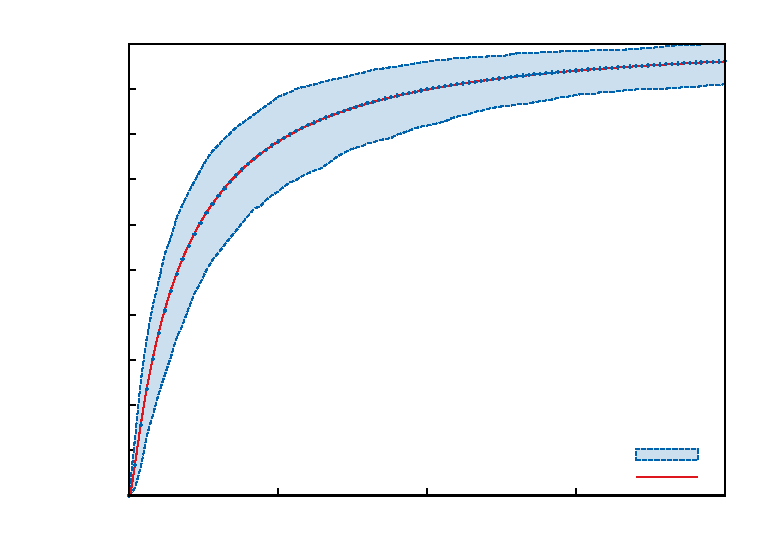
\includegraphics{./figures/elkc_exp_1D_lognormal_1}}%
    \gplfronttext
  \end{picture}%
\endgroup
}}\hspace*{\fill}
  \caption{Expectation of LKC for $\Msize=100$, $\mean=0.5$, $\std^2=2$, $\Lc=0.5$, and $\HS=\zu$ (log-normal distribution with cumulative hitting set) in 1D. Experimental results are calculated over $1\,000$ realizations.}
\end{figure}

\newpage 
\subsection{Two dimensions}
\begin{subequations}
\begin{align}
  &\Expec\left\{\LKC_0^\ES\right\} = \frac{\SpecMom}{2\pi}\LKC_2^\MRF\GMFk_2 + \sqrt{\frac{\SpecMom}{2\pi}}\LKC_1^\MRF\GMFk_1 + \LKC_0^\MRF\GMFk_0\\
  &\Expec\left\{\LKC_1^\ES\right\} = \sqrt{\frac{\SpecMom\pi}{8}}\LKC_2^\MRF\GMFk_1 + \LKC_1^\MRF\GMFk_0\\
  &\Expec\left\{\LKC_2^\ES\right\} = \LKC_2^\MRF\GMFk_0
\end{align}
\end{subequations}


\begin{figure}[!h]
  \centering
  \hspace*{\fill}
  \subfigure{\scalebox{0.5}{% GNUPLOT: LaTeX picture with Postscript
\begingroup
  \makeatletter
  \providecommand\color[2][]{%
    \GenericError{(gnuplot) \space\space\space\@spaces}{%
      Package color not loaded in conjunction with
      terminal option `colourtext'%
    }{See the gnuplot documentation for explanation.%
    }{Either use 'blacktext' in gnuplot or load the package
      color.sty in LaTeX.}%
    \renewcommand\color[2][]{}%
  }%
  \providecommand\includegraphics[2][]{%
    \GenericError{(gnuplot) \space\space\space\@spaces}{%
      Package graphicx or graphics not loaded%
    }{See the gnuplot documentation for explanation.%
    }{The gnuplot epslatex terminal needs graphicx.sty or graphics.sty.}%
    \renewcommand\includegraphics[2][]{}%
  }%
  \providecommand\rotatebox[2]{#2}%
  \@ifundefined{ifGPcolor}{%
    \newif\ifGPcolor
    \GPcolorfalse
  }{}%
  \@ifundefined{ifGPblacktext}{%
    \newif\ifGPblacktext
    \GPblacktexttrue
  }{}%
  % define a \g@addto@macro without @ in the name:
  \let\gplgaddtomacro\g@addto@macro
  % define empty templates for all commands taking text:
  \gdef\gplbacktext{}%
  \gdef\gplfronttext{}%
  \makeatother
  \ifGPblacktext
    % no textcolor at all
    \def\colorrgb#1{}%
    \def\colorgray#1{}%
  \else
    % gray or color?
    \ifGPcolor
      \def\colorrgb#1{\color[rgb]{#1}}%
      \def\colorgray#1{\color[gray]{#1}}%
      \expandafter\def\csname LTw\endcsname{\color{white}}%
      \expandafter\def\csname LTb\endcsname{\color{black}}%
      \expandafter\def\csname LTa\endcsname{\color{black}}%
      \expandafter\def\csname LT0\endcsname{\color[rgb]{1,0,0}}%
      \expandafter\def\csname LT1\endcsname{\color[rgb]{0,1,0}}%
      \expandafter\def\csname LT2\endcsname{\color[rgb]{0,0,1}}%
      \expandafter\def\csname LT3\endcsname{\color[rgb]{1,0,1}}%
      \expandafter\def\csname LT4\endcsname{\color[rgb]{0,1,1}}%
      \expandafter\def\csname LT5\endcsname{\color[rgb]{1,1,0}}%
      \expandafter\def\csname LT6\endcsname{\color[rgb]{0,0,0}}%
      \expandafter\def\csname LT7\endcsname{\color[rgb]{1,0.3,0}}%
      \expandafter\def\csname LT8\endcsname{\color[rgb]{0.5,0.5,0.5}}%
    \else
      % gray
      \def\colorrgb#1{\color{black}}%
      \def\colorgray#1{\color[gray]{#1}}%
      \expandafter\def\csname LTw\endcsname{\color{white}}%
      \expandafter\def\csname LTb\endcsname{\color{black}}%
      \expandafter\def\csname LTa\endcsname{\color{black}}%
      \expandafter\def\csname LT0\endcsname{\color{black}}%
      \expandafter\def\csname LT1\endcsname{\color{black}}%
      \expandafter\def\csname LT2\endcsname{\color{black}}%
      \expandafter\def\csname LT3\endcsname{\color{black}}%
      \expandafter\def\csname LT4\endcsname{\color{black}}%
      \expandafter\def\csname LT5\endcsname{\color{black}}%
      \expandafter\def\csname LT6\endcsname{\color{black}}%
      \expandafter\def\csname LT7\endcsname{\color{black}}%
      \expandafter\def\csname LT8\endcsname{\color{black}}%
    \fi
  \fi
  \setlength{\unitlength}{0.0500bp}%
  \begin{picture}(7200.00,5040.00)%
    \gplgaddtomacro\gplbacktext{%
      \csname LTb\endcsname%
      \put(814,704){\makebox(0,0)[r]{\strut{}-40}}%
      \put(814,1111){\makebox(0,0)[r]{\strut{}-30}}%
      \put(814,1518){\makebox(0,0)[r]{\strut{}-20}}%
      \put(814,1925){\makebox(0,0)[r]{\strut{}-10}}%
      \put(814,2332){\makebox(0,0)[r]{\strut{} 0}}%
      \put(814,2740){\makebox(0,0)[r]{\strut{} 10}}%
      \put(814,3147){\makebox(0,0)[r]{\strut{} 20}}%
      \put(814,3554){\makebox(0,0)[r]{\strut{} 30}}%
      \put(814,3961){\makebox(0,0)[r]{\strut{} 40}}%
      \put(814,4368){\makebox(0,0)[r]{\strut{} 50}}%
      \put(814,4775){\makebox(0,0)[r]{\strut{} 60}}%
      \put(946,484){\makebox(0,0){\strut{}-4}}%
      \put(1678,484){\makebox(0,0){\strut{}-3}}%
      \put(2410,484){\makebox(0,0){\strut{}-2}}%
      \put(3142,484){\makebox(0,0){\strut{}-1}}%
      \put(3875,484){\makebox(0,0){\strut{} 0}}%
      \put(4607,484){\makebox(0,0){\strut{} 1}}%
      \put(5339,484){\makebox(0,0){\strut{} 2}}%
      \put(6071,484){\makebox(0,0){\strut{} 3}}%
      \put(6803,484){\makebox(0,0){\strut{} 4}}%
      \csname LTb\endcsname%
      \put(176,2739){\rotatebox{90}{\makebox(0,0){\strut{}Euler characteristic}}}%
      \put(3874,154){\makebox(0,0){\strut{}$\lset$}}%
    }%
    \gplgaddtomacro\gplfronttext{%
      \csname LTb\endcsname%
      \put(2662,4602){\makebox(0,0)[r]{\strut{}Experimental}}%
      \csname LTb\endcsname%
      \put(2662,4382){\makebox(0,0)[r]{\strut{}Theoretical}}%
    }%
    \gplbacktext
    \put(0,0){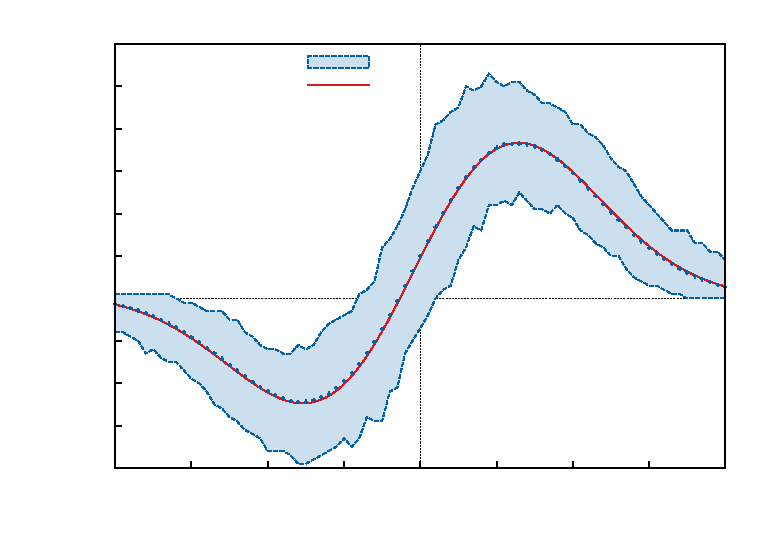
\includegraphics{./figures/elkc_exp_2D_gaussian_0}}%
    \gplfronttext
  \end{picture}%
\endgroup
}}\hfill
  \subfigure{\scalebox{0.5}{% GNUPLOT: LaTeX picture with Postscript
\begingroup
  \makeatletter
  \providecommand\color[2][]{%
    \GenericError{(gnuplot) \space\space\space\@spaces}{%
      Package color not loaded in conjunction with
      terminal option `colourtext'%
    }{See the gnuplot documentation for explanation.%
    }{Either use 'blacktext' in gnuplot or load the package
      color.sty in LaTeX.}%
    \renewcommand\color[2][]{}%
  }%
  \providecommand\includegraphics[2][]{%
    \GenericError{(gnuplot) \space\space\space\@spaces}{%
      Package graphicx or graphics not loaded%
    }{See the gnuplot documentation for explanation.%
    }{The gnuplot epslatex terminal needs graphicx.sty or graphics.sty.}%
    \renewcommand\includegraphics[2][]{}%
  }%
  \providecommand\rotatebox[2]{#2}%
  \@ifundefined{ifGPcolor}{%
    \newif\ifGPcolor
    \GPcolorfalse
  }{}%
  \@ifundefined{ifGPblacktext}{%
    \newif\ifGPblacktext
    \GPblacktexttrue
  }{}%
  % define a \g@addto@macro without @ in the name:
  \let\gplgaddtomacro\g@addto@macro
  % define empty templates for all commands taking text:
  \gdef\gplbacktext{}%
  \gdef\gplfronttext{}%
  \makeatother
  \ifGPblacktext
    % no textcolor at all
    \def\colorrgb#1{}%
    \def\colorgray#1{}%
  \else
    % gray or color?
    \ifGPcolor
      \def\colorrgb#1{\color[rgb]{#1}}%
      \def\colorgray#1{\color[gray]{#1}}%
      \expandafter\def\csname LTw\endcsname{\color{white}}%
      \expandafter\def\csname LTb\endcsname{\color{black}}%
      \expandafter\def\csname LTa\endcsname{\color{black}}%
      \expandafter\def\csname LT0\endcsname{\color[rgb]{1,0,0}}%
      \expandafter\def\csname LT1\endcsname{\color[rgb]{0,1,0}}%
      \expandafter\def\csname LT2\endcsname{\color[rgb]{0,0,1}}%
      \expandafter\def\csname LT3\endcsname{\color[rgb]{1,0,1}}%
      \expandafter\def\csname LT4\endcsname{\color[rgb]{0,1,1}}%
      \expandafter\def\csname LT5\endcsname{\color[rgb]{1,1,0}}%
      \expandafter\def\csname LT6\endcsname{\color[rgb]{0,0,0}}%
      \expandafter\def\csname LT7\endcsname{\color[rgb]{1,0.3,0}}%
      \expandafter\def\csname LT8\endcsname{\color[rgb]{0.5,0.5,0.5}}%
    \else
      % gray
      \def\colorrgb#1{\color{black}}%
      \def\colorgray#1{\color[gray]{#1}}%
      \expandafter\def\csname LTw\endcsname{\color{white}}%
      \expandafter\def\csname LTb\endcsname{\color{black}}%
      \expandafter\def\csname LTa\endcsname{\color{black}}%
      \expandafter\def\csname LT0\endcsname{\color{black}}%
      \expandafter\def\csname LT1\endcsname{\color{black}}%
      \expandafter\def\csname LT2\endcsname{\color{black}}%
      \expandafter\def\csname LT3\endcsname{\color{black}}%
      \expandafter\def\csname LT4\endcsname{\color{black}}%
      \expandafter\def\csname LT5\endcsname{\color{black}}%
      \expandafter\def\csname LT6\endcsname{\color{black}}%
      \expandafter\def\csname LT7\endcsname{\color{black}}%
      \expandafter\def\csname LT8\endcsname{\color{black}}%
    \fi
  \fi
  \setlength{\unitlength}{0.0500bp}%
  \begin{picture}(7200.00,5040.00)%
    \gplgaddtomacro\gplbacktext{%
      \csname LTb\endcsname%
      \put(946,704){\makebox(0,0)[r]{\strut{} 0}}%
      \put(946,1156){\makebox(0,0)[r]{\strut{} 100}}%
      \put(946,1609){\makebox(0,0)[r]{\strut{} 200}}%
      \put(946,2061){\makebox(0,0)[r]{\strut{} 300}}%
      \put(946,2513){\makebox(0,0)[r]{\strut{} 400}}%
      \put(946,2966){\makebox(0,0)[r]{\strut{} 500}}%
      \put(946,3418){\makebox(0,0)[r]{\strut{} 600}}%
      \put(946,3870){\makebox(0,0)[r]{\strut{} 700}}%
      \put(946,4323){\makebox(0,0)[r]{\strut{} 800}}%
      \put(946,4775){\makebox(0,0)[r]{\strut{} 900}}%
      \put(1078,484){\makebox(0,0){\strut{}-4}}%
      \put(1794,484){\makebox(0,0){\strut{}-3}}%
      \put(2509,484){\makebox(0,0){\strut{}-2}}%
      \put(3225,484){\makebox(0,0){\strut{}-1}}%
      \put(3941,484){\makebox(0,0){\strut{} 0}}%
      \put(4656,484){\makebox(0,0){\strut{} 1}}%
      \put(5372,484){\makebox(0,0){\strut{} 2}}%
      \put(6087,484){\makebox(0,0){\strut{} 3}}%
      \put(6803,484){\makebox(0,0){\strut{} 4}}%
      \csname LTb\endcsname%
      \put(176,2739){\rotatebox{90}{\makebox(0,0){\strut{}Half diameter}}}%
      \put(3940,154){\makebox(0,0){\strut{}$\lset$}}%
    }%
    \gplgaddtomacro\gplfronttext{%
      \csname LTb\endcsname%
      \put(5816,4602){\makebox(0,0)[r]{\strut{}Theoretical}}%
    }%
    \gplbacktext
    \put(0,0){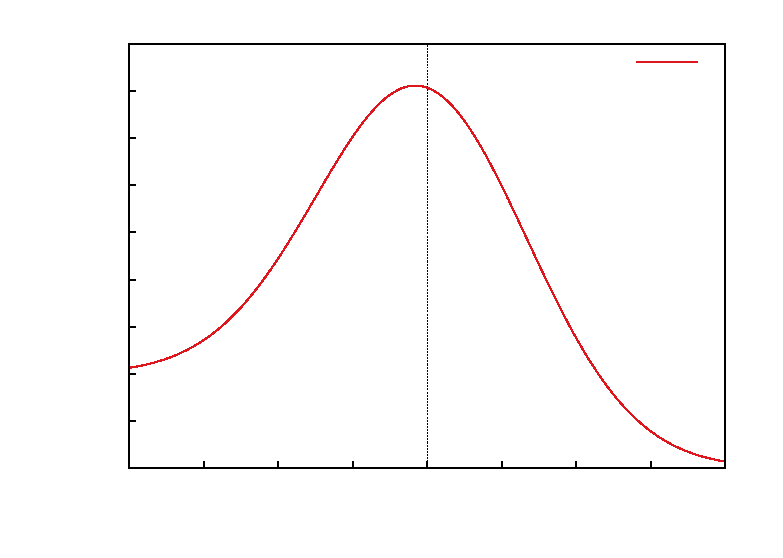
\includegraphics{./figures/elkc_exp_2D_gaussian_1}}%
    \gplfronttext
  \end{picture}%
\endgroup
}}\hfill
  \subfigure{\scalebox{0.5}{% GNUPLOT: LaTeX picture with Postscript
\begingroup
  \makeatletter
  \providecommand\color[2][]{%
    \GenericError{(gnuplot) \space\space\space\@spaces}{%
      Package color not loaded in conjunction with
      terminal option `colourtext'%
    }{See the gnuplot documentation for explanation.%
    }{Either use 'blacktext' in gnuplot or load the package
      color.sty in LaTeX.}%
    \renewcommand\color[2][]{}%
  }%
  \providecommand\includegraphics[2][]{%
    \GenericError{(gnuplot) \space\space\space\@spaces}{%
      Package graphicx or graphics not loaded%
    }{See the gnuplot documentation for explanation.%
    }{The gnuplot epslatex terminal needs graphicx.sty or graphics.sty.}%
    \renewcommand\includegraphics[2][]{}%
  }%
  \providecommand\rotatebox[2]{#2}%
  \@ifundefined{ifGPcolor}{%
    \newif\ifGPcolor
    \GPcolorfalse
  }{}%
  \@ifundefined{ifGPblacktext}{%
    \newif\ifGPblacktext
    \GPblacktexttrue
  }{}%
  % define a \g@addto@macro without @ in the name:
  \let\gplgaddtomacro\g@addto@macro
  % define empty templates for all commands taking text:
  \gdef\gplbacktext{}%
  \gdef\gplfronttext{}%
  \makeatother
  \ifGPblacktext
    % no textcolor at all
    \def\colorrgb#1{}%
    \def\colorgray#1{}%
  \else
    % gray or color?
    \ifGPcolor
      \def\colorrgb#1{\color[rgb]{#1}}%
      \def\colorgray#1{\color[gray]{#1}}%
      \expandafter\def\csname LTw\endcsname{\color{white}}%
      \expandafter\def\csname LTb\endcsname{\color{black}}%
      \expandafter\def\csname LTa\endcsname{\color{black}}%
      \expandafter\def\csname LT0\endcsname{\color[rgb]{1,0,0}}%
      \expandafter\def\csname LT1\endcsname{\color[rgb]{0,1,0}}%
      \expandafter\def\csname LT2\endcsname{\color[rgb]{0,0,1}}%
      \expandafter\def\csname LT3\endcsname{\color[rgb]{1,0,1}}%
      \expandafter\def\csname LT4\endcsname{\color[rgb]{0,1,1}}%
      \expandafter\def\csname LT5\endcsname{\color[rgb]{1,1,0}}%
      \expandafter\def\csname LT6\endcsname{\color[rgb]{0,0,0}}%
      \expandafter\def\csname LT7\endcsname{\color[rgb]{1,0.3,0}}%
      \expandafter\def\csname LT8\endcsname{\color[rgb]{0.5,0.5,0.5}}%
    \else
      % gray
      \def\colorrgb#1{\color{black}}%
      \def\colorgray#1{\color[gray]{#1}}%
      \expandafter\def\csname LTw\endcsname{\color{white}}%
      \expandafter\def\csname LTb\endcsname{\color{black}}%
      \expandafter\def\csname LTa\endcsname{\color{black}}%
      \expandafter\def\csname LT0\endcsname{\color{black}}%
      \expandafter\def\csname LT1\endcsname{\color{black}}%
      \expandafter\def\csname LT2\endcsname{\color{black}}%
      \expandafter\def\csname LT3\endcsname{\color{black}}%
      \expandafter\def\csname LT4\endcsname{\color{black}}%
      \expandafter\def\csname LT5\endcsname{\color{black}}%
      \expandafter\def\csname LT6\endcsname{\color{black}}%
      \expandafter\def\csname LT7\endcsname{\color{black}}%
      \expandafter\def\csname LT8\endcsname{\color{black}}%
    \fi
  \fi
  \setlength{\unitlength}{0.0500bp}%
  \begin{picture}(7200.00,5040.00)%
    \gplgaddtomacro\gplbacktext{%
      \csname LTb\endcsname%
      \put(1210,704){\makebox(0,0)[r]{\strut{} 0}}%
      \put(1210,1518){\makebox(0,0)[r]{\strut{} 2000}}%
      \put(1210,2332){\makebox(0,0)[r]{\strut{} 4000}}%
      \put(1210,3147){\makebox(0,0)[r]{\strut{} 6000}}%
      \put(1210,3961){\makebox(0,0)[r]{\strut{} 8000}}%
      \put(1210,4775){\makebox(0,0)[r]{\strut{} 10000}}%
      \put(1342,484){\makebox(0,0){\strut{}-4}}%
      \put(2025,484){\makebox(0,0){\strut{}-3}}%
      \put(2707,484){\makebox(0,0){\strut{}-2}}%
      \put(3390,484){\makebox(0,0){\strut{}-1}}%
      \put(4073,484){\makebox(0,0){\strut{} 0}}%
      \put(4755,484){\makebox(0,0){\strut{} 1}}%
      \put(5438,484){\makebox(0,0){\strut{} 2}}%
      \put(6120,484){\makebox(0,0){\strut{} 3}}%
      \put(6803,484){\makebox(0,0){\strut{} 4}}%
      \csname LTb\endcsname%
      \put(176,2739){\rotatebox{90}{\makebox(0,0){\strut{}Surface area}}}%
      \put(4072,154){\makebox(0,0){\strut{}$\lset$}}%
    }%
    \gplgaddtomacro\gplfronttext{%
      \csname LTb\endcsname%
      \put(5816,4602){\makebox(0,0)[r]{\strut{}Experimental}}%
      \csname LTb\endcsname%
      \put(5816,4382){\makebox(0,0)[r]{\strut{}Theoretical}}%
    }%
    \gplbacktext
    \put(0,0){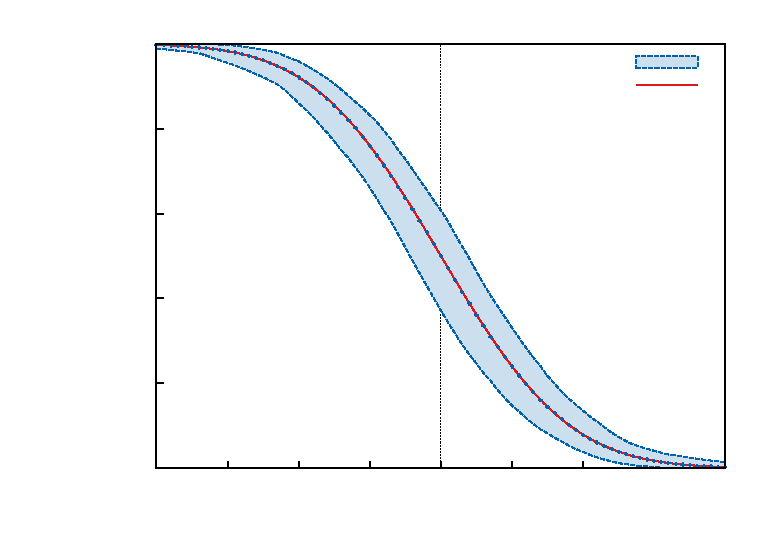
\includegraphics{./figures/elkc_exp_2D_gaussian_2}}%
    \gplfronttext
  \end{picture}%
\endgroup
}}\hspace*{\fill}
  \caption{Expectation of LKC for $\Msize=100$, $\mean=0.0$, $\std^2=2$, $\Lc=5$, and $\HS=\uinf$ (gaussian distribution with tail hitting set) in 2D. Experimental results are calculated over $1\,000$ realizations.}
\end{figure}

\begin{figure}[!h]
  \centering
  \hspace*{\fill}
  \subfigure{\scalebox{0.5}{% GNUPLOT: LaTeX picture with Postscript
\begingroup
  \makeatletter
  \providecommand\color[2][]{%
    \GenericError{(gnuplot) \space\space\space\@spaces}{%
      Package color not loaded in conjunction with
      terminal option `colourtext'%
    }{See the gnuplot documentation for explanation.%
    }{Either use 'blacktext' in gnuplot or load the package
      color.sty in LaTeX.}%
    \renewcommand\color[2][]{}%
  }%
  \providecommand\includegraphics[2][]{%
    \GenericError{(gnuplot) \space\space\space\@spaces}{%
      Package graphicx or graphics not loaded%
    }{See the gnuplot documentation for explanation.%
    }{The gnuplot epslatex terminal needs graphicx.sty or graphics.sty.}%
    \renewcommand\includegraphics[2][]{}%
  }%
  \providecommand\rotatebox[2]{#2}%
  \@ifundefined{ifGPcolor}{%
    \newif\ifGPcolor
    \GPcolorfalse
  }{}%
  \@ifundefined{ifGPblacktext}{%
    \newif\ifGPblacktext
    \GPblacktexttrue
  }{}%
  % define a \g@addto@macro without @ in the name:
  \let\gplgaddtomacro\g@addto@macro
  % define empty templates for all commands taking text:
  \gdef\gplbacktext{}%
  \gdef\gplfronttext{}%
  \makeatother
  \ifGPblacktext
    % no textcolor at all
    \def\colorrgb#1{}%
    \def\colorgray#1{}%
  \else
    % gray or color?
    \ifGPcolor
      \def\colorrgb#1{\color[rgb]{#1}}%
      \def\colorgray#1{\color[gray]{#1}}%
      \expandafter\def\csname LTw\endcsname{\color{white}}%
      \expandafter\def\csname LTb\endcsname{\color{black}}%
      \expandafter\def\csname LTa\endcsname{\color{black}}%
      \expandafter\def\csname LT0\endcsname{\color[rgb]{1,0,0}}%
      \expandafter\def\csname LT1\endcsname{\color[rgb]{0,1,0}}%
      \expandafter\def\csname LT2\endcsname{\color[rgb]{0,0,1}}%
      \expandafter\def\csname LT3\endcsname{\color[rgb]{1,0,1}}%
      \expandafter\def\csname LT4\endcsname{\color[rgb]{0,1,1}}%
      \expandafter\def\csname LT5\endcsname{\color[rgb]{1,1,0}}%
      \expandafter\def\csname LT6\endcsname{\color[rgb]{0,0,0}}%
      \expandafter\def\csname LT7\endcsname{\color[rgb]{1,0.3,0}}%
      \expandafter\def\csname LT8\endcsname{\color[rgb]{0.5,0.5,0.5}}%
    \else
      % gray
      \def\colorrgb#1{\color{black}}%
      \def\colorgray#1{\color[gray]{#1}}%
      \expandafter\def\csname LTw\endcsname{\color{white}}%
      \expandafter\def\csname LTb\endcsname{\color{black}}%
      \expandafter\def\csname LTa\endcsname{\color{black}}%
      \expandafter\def\csname LT0\endcsname{\color{black}}%
      \expandafter\def\csname LT1\endcsname{\color{black}}%
      \expandafter\def\csname LT2\endcsname{\color{black}}%
      \expandafter\def\csname LT3\endcsname{\color{black}}%
      \expandafter\def\csname LT4\endcsname{\color{black}}%
      \expandafter\def\csname LT5\endcsname{\color{black}}%
      \expandafter\def\csname LT6\endcsname{\color{black}}%
      \expandafter\def\csname LT7\endcsname{\color{black}}%
      \expandafter\def\csname LT8\endcsname{\color{black}}%
    \fi
  \fi
  \setlength{\unitlength}{0.0500bp}%
  \begin{picture}(7200.00,5040.00)%
    \gplgaddtomacro\gplbacktext{%
      \csname LTb\endcsname%
      \put(814,704){\makebox(0,0)[r]{\strut{}-40}}%
      \put(814,1111){\makebox(0,0)[r]{\strut{}-30}}%
      \put(814,1518){\makebox(0,0)[r]{\strut{}-20}}%
      \put(814,1925){\makebox(0,0)[r]{\strut{}-10}}%
      \put(814,2332){\makebox(0,0)[r]{\strut{} 0}}%
      \put(814,2740){\makebox(0,0)[r]{\strut{} 10}}%
      \put(814,3147){\makebox(0,0)[r]{\strut{} 20}}%
      \put(814,3554){\makebox(0,0)[r]{\strut{} 30}}%
      \put(814,3961){\makebox(0,0)[r]{\strut{} 40}}%
      \put(814,4368){\makebox(0,0)[r]{\strut{} 50}}%
      \put(814,4775){\makebox(0,0)[r]{\strut{} 60}}%
      \put(946,484){\makebox(0,0){\strut{} 0.01}}%
      \put(2117,484){\makebox(0,0){\strut{} 0.1}}%
      \put(3289,484){\makebox(0,0){\strut{} 1}}%
      \put(4460,484){\makebox(0,0){\strut{} 10}}%
      \put(5632,484){\makebox(0,0){\strut{} 100}}%
      \put(6803,484){\makebox(0,0){\strut{} 1000}}%
      \csname LTb\endcsname%
      \put(176,2739){\rotatebox{90}{\makebox(0,0){\strut{}Euler characteristic}}}%
      \put(3874,154){\makebox(0,0){\strut{}$\lset$}}%
    }%
    \gplgaddtomacro\gplfronttext{%
      \csname LTb\endcsname%
      \put(5816,4602){\makebox(0,0)[r]{\strut{}Experimental}}%
      \csname LTb\endcsname%
      \put(5816,4382){\makebox(0,0)[r]{\strut{}Theoretical}}%
    }%
    \gplbacktext
    \put(0,0){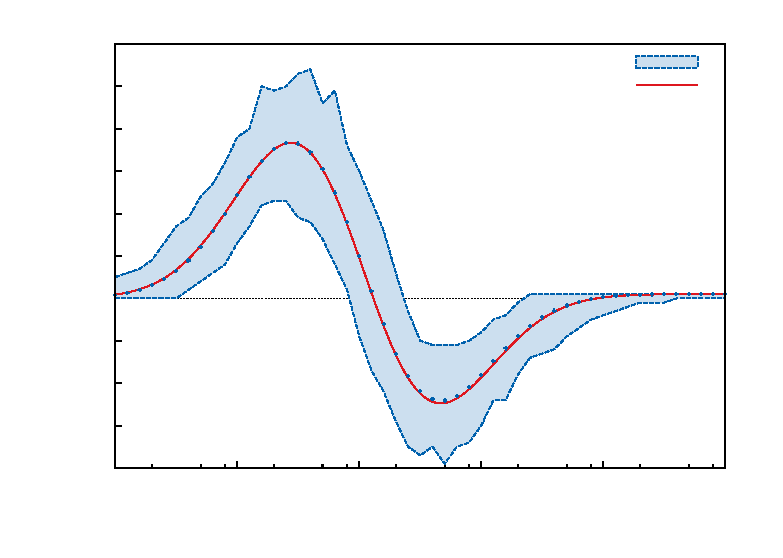
\includegraphics{./figures/elkc_exp_2D_lognormal_0}}%
    \gplfronttext
  \end{picture}%
\endgroup
}}\hfill
  \subfigure{\scalebox{0.5}{% GNUPLOT: LaTeX picture with Postscript
\begingroup
  \makeatletter
  \providecommand\color[2][]{%
    \GenericError{(gnuplot) \space\space\space\@spaces}{%
      Package color not loaded in conjunction with
      terminal option `colourtext'%
    }{See the gnuplot documentation for explanation.%
    }{Either use 'blacktext' in gnuplot or load the package
      color.sty in LaTeX.}%
    \renewcommand\color[2][]{}%
  }%
  \providecommand\includegraphics[2][]{%
    \GenericError{(gnuplot) \space\space\space\@spaces}{%
      Package graphicx or graphics not loaded%
    }{See the gnuplot documentation for explanation.%
    }{The gnuplot epslatex terminal needs graphicx.sty or graphics.sty.}%
    \renewcommand\includegraphics[2][]{}%
  }%
  \providecommand\rotatebox[2]{#2}%
  \@ifundefined{ifGPcolor}{%
    \newif\ifGPcolor
    \GPcolorfalse
  }{}%
  \@ifundefined{ifGPblacktext}{%
    \newif\ifGPblacktext
    \GPblacktexttrue
  }{}%
  % define a \g@addto@macro without @ in the name:
  \let\gplgaddtomacro\g@addto@macro
  % define empty templates for all commands taking text:
  \gdef\gplbacktext{}%
  \gdef\gplfronttext{}%
  \makeatother
  \ifGPblacktext
    % no textcolor at all
    \def\colorrgb#1{}%
    \def\colorgray#1{}%
  \else
    % gray or color?
    \ifGPcolor
      \def\colorrgb#1{\color[rgb]{#1}}%
      \def\colorgray#1{\color[gray]{#1}}%
      \expandafter\def\csname LTw\endcsname{\color{white}}%
      \expandafter\def\csname LTb\endcsname{\color{black}}%
      \expandafter\def\csname LTa\endcsname{\color{black}}%
      \expandafter\def\csname LT0\endcsname{\color[rgb]{1,0,0}}%
      \expandafter\def\csname LT1\endcsname{\color[rgb]{0,1,0}}%
      \expandafter\def\csname LT2\endcsname{\color[rgb]{0,0,1}}%
      \expandafter\def\csname LT3\endcsname{\color[rgb]{1,0,1}}%
      \expandafter\def\csname LT4\endcsname{\color[rgb]{0,1,1}}%
      \expandafter\def\csname LT5\endcsname{\color[rgb]{1,1,0}}%
      \expandafter\def\csname LT6\endcsname{\color[rgb]{0,0,0}}%
      \expandafter\def\csname LT7\endcsname{\color[rgb]{1,0.3,0}}%
      \expandafter\def\csname LT8\endcsname{\color[rgb]{0.5,0.5,0.5}}%
    \else
      % gray
      \def\colorrgb#1{\color{black}}%
      \def\colorgray#1{\color[gray]{#1}}%
      \expandafter\def\csname LTw\endcsname{\color{white}}%
      \expandafter\def\csname LTb\endcsname{\color{black}}%
      \expandafter\def\csname LTa\endcsname{\color{black}}%
      \expandafter\def\csname LT0\endcsname{\color{black}}%
      \expandafter\def\csname LT1\endcsname{\color{black}}%
      \expandafter\def\csname LT2\endcsname{\color{black}}%
      \expandafter\def\csname LT3\endcsname{\color{black}}%
      \expandafter\def\csname LT4\endcsname{\color{black}}%
      \expandafter\def\csname LT5\endcsname{\color{black}}%
      \expandafter\def\csname LT6\endcsname{\color{black}}%
      \expandafter\def\csname LT7\endcsname{\color{black}}%
      \expandafter\def\csname LT8\endcsname{\color{black}}%
    \fi
  \fi
  \setlength{\unitlength}{0.0500bp}%
  \begin{picture}(7200.00,5040.00)%
    \gplgaddtomacro\gplbacktext{%
      \csname LTb\endcsname%
      \put(946,704){\makebox(0,0)[r]{\strut{} 0}}%
      \put(946,1156){\makebox(0,0)[r]{\strut{} 100}}%
      \put(946,1609){\makebox(0,0)[r]{\strut{} 200}}%
      \put(946,2061){\makebox(0,0)[r]{\strut{} 300}}%
      \put(946,2513){\makebox(0,0)[r]{\strut{} 400}}%
      \put(946,2966){\makebox(0,0)[r]{\strut{} 500}}%
      \put(946,3418){\makebox(0,0)[r]{\strut{} 600}}%
      \put(946,3870){\makebox(0,0)[r]{\strut{} 700}}%
      \put(946,4323){\makebox(0,0)[r]{\strut{} 800}}%
      \put(946,4775){\makebox(0,0)[r]{\strut{} 900}}%
      \put(1078,484){\makebox(0,0){\strut{} 0.01}}%
      \put(2223,484){\makebox(0,0){\strut{} 0.1}}%
      \put(3368,484){\makebox(0,0){\strut{} 1}}%
      \put(4513,484){\makebox(0,0){\strut{} 10}}%
      \put(5658,484){\makebox(0,0){\strut{} 100}}%
      \put(6803,484){\makebox(0,0){\strut{} 1000}}%
      \csname LTb\endcsname%
      \put(176,2739){\rotatebox{90}{\makebox(0,0){\strut{}Half diameter}}}%
      \put(3940,154){\makebox(0,0){\strut{}$\lset$}}%
    }%
    \gplgaddtomacro\gplfronttext{%
      \csname LTb\endcsname%
      \put(5816,4602){\makebox(0,0)[r]{\strut{}Theoretical}}%
    }%
    \gplbacktext
    \put(0,0){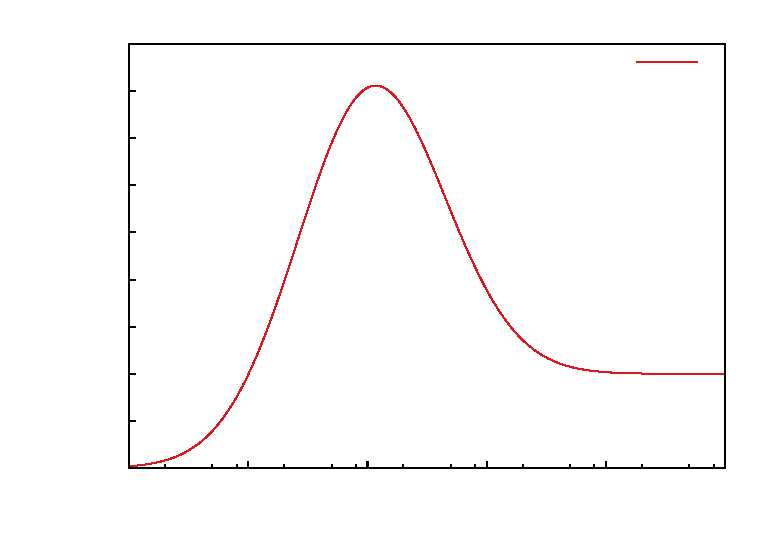
\includegraphics{./figures/elkc_exp_2D_lognormal_1}}%
    \gplfronttext
  \end{picture}%
\endgroup
}}\hfill
  \subfigure{\scalebox{0.5}{% GNUPLOT: LaTeX picture with Postscript
\begingroup
  \makeatletter
  \providecommand\color[2][]{%
    \GenericError{(gnuplot) \space\space\space\@spaces}{%
      Package color not loaded in conjunction with
      terminal option `colourtext'%
    }{See the gnuplot documentation for explanation.%
    }{Either use 'blacktext' in gnuplot or load the package
      color.sty in LaTeX.}%
    \renewcommand\color[2][]{}%
  }%
  \providecommand\includegraphics[2][]{%
    \GenericError{(gnuplot) \space\space\space\@spaces}{%
      Package graphicx or graphics not loaded%
    }{See the gnuplot documentation for explanation.%
    }{The gnuplot epslatex terminal needs graphicx.sty or graphics.sty.}%
    \renewcommand\includegraphics[2][]{}%
  }%
  \providecommand\rotatebox[2]{#2}%
  \@ifundefined{ifGPcolor}{%
    \newif\ifGPcolor
    \GPcolorfalse
  }{}%
  \@ifundefined{ifGPblacktext}{%
    \newif\ifGPblacktext
    \GPblacktexttrue
  }{}%
  % define a \g@addto@macro without @ in the name:
  \let\gplgaddtomacro\g@addto@macro
  % define empty templates for all commands taking text:
  \gdef\gplbacktext{}%
  \gdef\gplfronttext{}%
  \makeatother
  \ifGPblacktext
    % no textcolor at all
    \def\colorrgb#1{}%
    \def\colorgray#1{}%
  \else
    % gray or color?
    \ifGPcolor
      \def\colorrgb#1{\color[rgb]{#1}}%
      \def\colorgray#1{\color[gray]{#1}}%
      \expandafter\def\csname LTw\endcsname{\color{white}}%
      \expandafter\def\csname LTb\endcsname{\color{black}}%
      \expandafter\def\csname LTa\endcsname{\color{black}}%
      \expandafter\def\csname LT0\endcsname{\color[rgb]{1,0,0}}%
      \expandafter\def\csname LT1\endcsname{\color[rgb]{0,1,0}}%
      \expandafter\def\csname LT2\endcsname{\color[rgb]{0,0,1}}%
      \expandafter\def\csname LT3\endcsname{\color[rgb]{1,0,1}}%
      \expandafter\def\csname LT4\endcsname{\color[rgb]{0,1,1}}%
      \expandafter\def\csname LT5\endcsname{\color[rgb]{1,1,0}}%
      \expandafter\def\csname LT6\endcsname{\color[rgb]{0,0,0}}%
      \expandafter\def\csname LT7\endcsname{\color[rgb]{1,0.3,0}}%
      \expandafter\def\csname LT8\endcsname{\color[rgb]{0.5,0.5,0.5}}%
    \else
      % gray
      \def\colorrgb#1{\color{black}}%
      \def\colorgray#1{\color[gray]{#1}}%
      \expandafter\def\csname LTw\endcsname{\color{white}}%
      \expandafter\def\csname LTb\endcsname{\color{black}}%
      \expandafter\def\csname LTa\endcsname{\color{black}}%
      \expandafter\def\csname LT0\endcsname{\color{black}}%
      \expandafter\def\csname LT1\endcsname{\color{black}}%
      \expandafter\def\csname LT2\endcsname{\color{black}}%
      \expandafter\def\csname LT3\endcsname{\color{black}}%
      \expandafter\def\csname LT4\endcsname{\color{black}}%
      \expandafter\def\csname LT5\endcsname{\color{black}}%
      \expandafter\def\csname LT6\endcsname{\color{black}}%
      \expandafter\def\csname LT7\endcsname{\color{black}}%
      \expandafter\def\csname LT8\endcsname{\color{black}}%
    \fi
  \fi
  \setlength{\unitlength}{0.0500bp}%
  \begin{picture}(7200.00,5040.00)%
    \gplgaddtomacro\gplbacktext{%
      \csname LTb\endcsname%
      \put(1210,704){\makebox(0,0)[r]{\strut{} 0}}%
      \put(1210,1518){\makebox(0,0)[r]{\strut{} 2000}}%
      \put(1210,2332){\makebox(0,0)[r]{\strut{} 4000}}%
      \put(1210,3147){\makebox(0,0)[r]{\strut{} 6000}}%
      \put(1210,3961){\makebox(0,0)[r]{\strut{} 8000}}%
      \put(1210,4775){\makebox(0,0)[r]{\strut{} 10000}}%
      \put(1342,484){\makebox(0,0){\strut{} 0.01}}%
      \put(2434,484){\makebox(0,0){\strut{} 0.1}}%
      \put(3526,484){\makebox(0,0){\strut{} 1}}%
      \put(4619,484){\makebox(0,0){\strut{} 10}}%
      \put(5711,484){\makebox(0,0){\strut{} 100}}%
      \put(6803,484){\makebox(0,0){\strut{} 1000}}%
      \csname LTb\endcsname%
      \put(176,2739){\rotatebox{90}{\makebox(0,0){\strut{}Surface area}}}%
      \put(4072,154){\makebox(0,0){\strut{}$\lset$}}%
    }%
    \gplgaddtomacro\gplfronttext{%
      \csname LTb\endcsname%
      \put(3058,4602){\makebox(0,0)[r]{\strut{}Experimental}}%
      \csname LTb\endcsname%
      \put(3058,4382){\makebox(0,0)[r]{\strut{}Theoretical}}%
    }%
    \gplbacktext
    \put(0,0){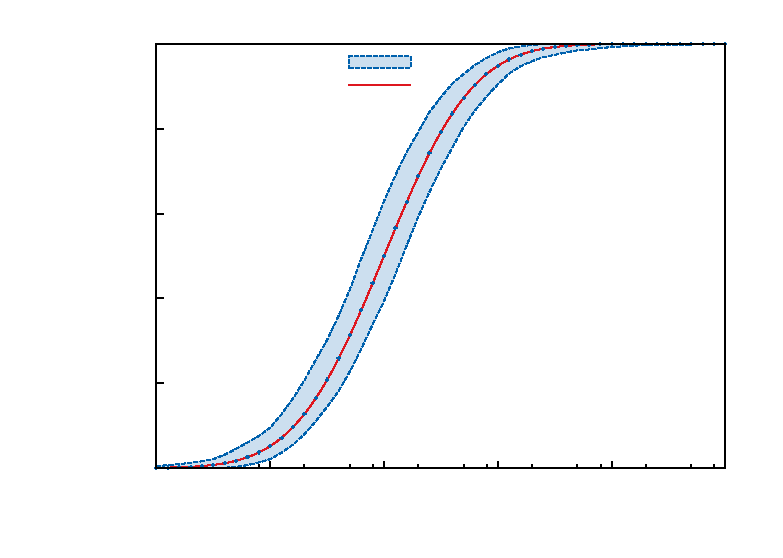
\includegraphics{./figures/elkc_exp_2D_lognormal_2}}%
    \gplfronttext
  \end{picture}%
\endgroup
}}\hspace*{\fill}
  \caption{Expectation of LKC for $\Msize=100$, $\mean=0.0$, $\std^2=2$, $\Lc=5$, and $\HS=\zu$ (lognormal distribution with cumulative hitting set) in 2D. Experimental results are calculated over $1\,000$ realizations.}
\end{figure}

\newpage
\subsubsection{Three dimensions}
\begin{subequations}
\begin{align}
  \Expec\left\{\LKC_0^\ES\right\} &= \left(\frac{\SpecMom}{2\pi}\right)^\frac{3}{2}\LKC_3^\MRF\GMFk_3 +\frac{\SpecMom}{2\pi}\LKC_2^\MRF\GMFk_2 + \left(\frac{\SpecMom}{2\pi}\right)^\frac{1}{2}\LKC_1^\MRF\GMFk_1 + \LKC_0^\MRF\GMFk_0\\
  \Expec\left\{\LKC_1^\ES\right\} &= \frac{\SpecMom}{\pi}\LKC_3^\MRF\GMFk_2 + \frac{\sqrt{\SpecMom\pi}}{2\sqrt{2}}\LKC_2^\MRF\GMFk_1 + \LKC_1^\MRF\GMFk_0\\
  \Expec\left\{\LKC_2^\ES\right\} &= \sqrt{\frac{2\SpecMom}{\pi}}\LKC_3^\MRF\GMFk_1 + \LKC_2^\MRF\GMFk_0\\
  \Expec\left\{\LKC_3^\ES\right\} &= \LKC_3^\MRF\GMFk_0
\end{align}
\end{subequations}


\begin{figure}[!h]
  \centering
  \subfigure{\scalebox{0.5}{% GNUPLOT: LaTeX picture with Postscript
\begingroup
  \makeatletter
  \providecommand\color[2][]{%
    \GenericError{(gnuplot) \space\space\space\@spaces}{%
      Package color not loaded in conjunction with
      terminal option `colourtext'%
    }{See the gnuplot documentation for explanation.%
    }{Either use 'blacktext' in gnuplot or load the package
      color.sty in LaTeX.}%
    \renewcommand\color[2][]{}%
  }%
  \providecommand\includegraphics[2][]{%
    \GenericError{(gnuplot) \space\space\space\@spaces}{%
      Package graphicx or graphics not loaded%
    }{See the gnuplot documentation for explanation.%
    }{The gnuplot epslatex terminal needs graphicx.sty or graphics.sty.}%
    \renewcommand\includegraphics[2][]{}%
  }%
  \providecommand\rotatebox[2]{#2}%
  \@ifundefined{ifGPcolor}{%
    \newif\ifGPcolor
    \GPcolorfalse
  }{}%
  \@ifundefined{ifGPblacktext}{%
    \newif\ifGPblacktext
    \GPblacktexttrue
  }{}%
  % define a \g@addto@macro without @ in the name:
  \let\gplgaddtomacro\g@addto@macro
  % define empty templates for all commands taking text:
  \gdef\gplbacktext{}%
  \gdef\gplfronttext{}%
  \makeatother
  \ifGPblacktext
    % no textcolor at all
    \def\colorrgb#1{}%
    \def\colorgray#1{}%
  \else
    % gray or color?
    \ifGPcolor
      \def\colorrgb#1{\color[rgb]{#1}}%
      \def\colorgray#1{\color[gray]{#1}}%
      \expandafter\def\csname LTw\endcsname{\color{white}}%
      \expandafter\def\csname LTb\endcsname{\color{black}}%
      \expandafter\def\csname LTa\endcsname{\color{black}}%
      \expandafter\def\csname LT0\endcsname{\color[rgb]{1,0,0}}%
      \expandafter\def\csname LT1\endcsname{\color[rgb]{0,1,0}}%
      \expandafter\def\csname LT2\endcsname{\color[rgb]{0,0,1}}%
      \expandafter\def\csname LT3\endcsname{\color[rgb]{1,0,1}}%
      \expandafter\def\csname LT4\endcsname{\color[rgb]{0,1,1}}%
      \expandafter\def\csname LT5\endcsname{\color[rgb]{1,1,0}}%
      \expandafter\def\csname LT6\endcsname{\color[rgb]{0,0,0}}%
      \expandafter\def\csname LT7\endcsname{\color[rgb]{1,0.3,0}}%
      \expandafter\def\csname LT8\endcsname{\color[rgb]{0.5,0.5,0.5}}%
    \else
      % gray
      \def\colorrgb#1{\color{black}}%
      \def\colorgray#1{\color[gray]{#1}}%
      \expandafter\def\csname LTw\endcsname{\color{white}}%
      \expandafter\def\csname LTb\endcsname{\color{black}}%
      \expandafter\def\csname LTa\endcsname{\color{black}}%
      \expandafter\def\csname LT0\endcsname{\color{black}}%
      \expandafter\def\csname LT1\endcsname{\color{black}}%
      \expandafter\def\csname LT2\endcsname{\color{black}}%
      \expandafter\def\csname LT3\endcsname{\color{black}}%
      \expandafter\def\csname LT4\endcsname{\color{black}}%
      \expandafter\def\csname LT5\endcsname{\color{black}}%
      \expandafter\def\csname LT6\endcsname{\color{black}}%
      \expandafter\def\csname LT7\endcsname{\color{black}}%
      \expandafter\def\csname LT8\endcsname{\color{black}}%
    \fi
  \fi
  \setlength{\unitlength}{0.0500bp}%
  \begin{picture}(7200.00,5040.00)%
    \gplgaddtomacro\gplbacktext{%
      \csname LTb\endcsname%
      \put(946,704){\makebox(0,0)[r]{\strut{}-400}}%
      \put(946,1286){\makebox(0,0)[r]{\strut{}-300}}%
      \put(946,1867){\makebox(0,0)[r]{\strut{}-200}}%
      \put(946,2449){\makebox(0,0)[r]{\strut{}-100}}%
      \put(946,3030){\makebox(0,0)[r]{\strut{} 0}}%
      \put(946,3612){\makebox(0,0)[r]{\strut{} 100}}%
      \put(946,4193){\makebox(0,0)[r]{\strut{} 200}}%
      \put(946,4775){\makebox(0,0)[r]{\strut{} 300}}%
      \put(1651,484){\makebox(0,0){\strut{}-4}}%
      \put(2796,484){\makebox(0,0){\strut{}-2}}%
      \put(3941,484){\makebox(0,0){\strut{} 0}}%
      \put(5086,484){\makebox(0,0){\strut{} 2}}%
      \put(6231,484){\makebox(0,0){\strut{} 4}}%
      \csname LTb\endcsname%
      \put(176,2739){\rotatebox{90}{\makebox(0,0){\strut{}Euler characteristic}}}%
      \put(3940,154){\makebox(0,0){\strut{}$\lset$}}%
    }%
    \gplgaddtomacro\gplfronttext{%
      \csname LTb\endcsname%
      \put(2794,4602){\makebox(0,0)[r]{\strut{}Experimental}}%
      \csname LTb\endcsname%
      \put(2794,4382){\makebox(0,0)[r]{\strut{}Theoretical}}%
    }%
    \gplbacktext
    \put(0,0){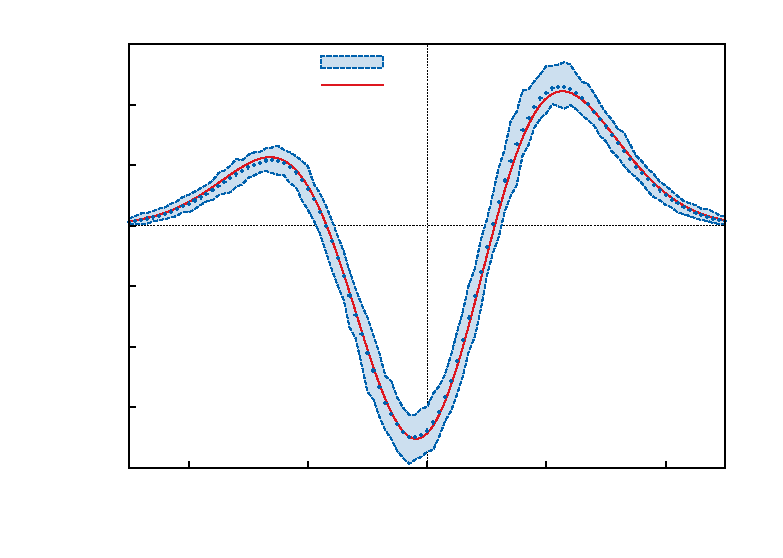
\includegraphics{./figures/elkc_exp_3D_gaussian_0}}%
    \gplfronttext
  \end{picture}%
\endgroup
}}\hspace{1.2cm}
  \subfigure{\scalebox{0.5}{% GNUPLOT: LaTeX picture with Postscript
\begingroup
  \makeatletter
  \providecommand\color[2][]{%
    \GenericError{(gnuplot) \space\space\space\@spaces}{%
      Package color not loaded in conjunction with
      terminal option `colourtext'%
    }{See the gnuplot documentation for explanation.%
    }{Either use 'blacktext' in gnuplot or load the package
      color.sty in LaTeX.}%
    \renewcommand\color[2][]{}%
  }%
  \providecommand\includegraphics[2][]{%
    \GenericError{(gnuplot) \space\space\space\@spaces}{%
      Package graphicx or graphics not loaded%
    }{See the gnuplot documentation for explanation.%
    }{The gnuplot epslatex terminal needs graphicx.sty or graphics.sty.}%
    \renewcommand\includegraphics[2][]{}%
  }%
  \providecommand\rotatebox[2]{#2}%
  \@ifundefined{ifGPcolor}{%
    \newif\ifGPcolor
    \GPcolorfalse
  }{}%
  \@ifundefined{ifGPblacktext}{%
    \newif\ifGPblacktext
    \GPblacktexttrue
  }{}%
  % define a \g@addto@macro without @ in the name:
  \let\gplgaddtomacro\g@addto@macro
  % define empty templates for all commands taking text:
  \gdef\gplbacktext{}%
  \gdef\gplfronttext{}%
  \makeatother
  \ifGPblacktext
    % no textcolor at all
    \def\colorrgb#1{}%
    \def\colorgray#1{}%
  \else
    % gray or color?
    \ifGPcolor
      \def\colorrgb#1{\color[rgb]{#1}}%
      \def\colorgray#1{\color[gray]{#1}}%
      \expandafter\def\csname LTw\endcsname{\color{white}}%
      \expandafter\def\csname LTb\endcsname{\color{black}}%
      \expandafter\def\csname LTa\endcsname{\color{black}}%
      \expandafter\def\csname LT0\endcsname{\color[rgb]{1,0,0}}%
      \expandafter\def\csname LT1\endcsname{\color[rgb]{0,1,0}}%
      \expandafter\def\csname LT2\endcsname{\color[rgb]{0,0,1}}%
      \expandafter\def\csname LT3\endcsname{\color[rgb]{1,0,1}}%
      \expandafter\def\csname LT4\endcsname{\color[rgb]{0,1,1}}%
      \expandafter\def\csname LT5\endcsname{\color[rgb]{1,1,0}}%
      \expandafter\def\csname LT6\endcsname{\color[rgb]{0,0,0}}%
      \expandafter\def\csname LT7\endcsname{\color[rgb]{1,0.3,0}}%
      \expandafter\def\csname LT8\endcsname{\color[rgb]{0.5,0.5,0.5}}%
    \else
      % gray
      \def\colorrgb#1{\color{black}}%
      \def\colorgray#1{\color[gray]{#1}}%
      \expandafter\def\csname LTw\endcsname{\color{white}}%
      \expandafter\def\csname LTb\endcsname{\color{black}}%
      \expandafter\def\csname LTa\endcsname{\color{black}}%
      \expandafter\def\csname LT0\endcsname{\color{black}}%
      \expandafter\def\csname LT1\endcsname{\color{black}}%
      \expandafter\def\csname LT2\endcsname{\color{black}}%
      \expandafter\def\csname LT3\endcsname{\color{black}}%
      \expandafter\def\csname LT4\endcsname{\color{black}}%
      \expandafter\def\csname LT5\endcsname{\color{black}}%
      \expandafter\def\csname LT6\endcsname{\color{black}}%
      \expandafter\def\csname LT7\endcsname{\color{black}}%
      \expandafter\def\csname LT8\endcsname{\color{black}}%
    \fi
  \fi
  \setlength{\unitlength}{0.0500bp}%
  \begin{picture}(7200.00,5040.00)%
    \gplgaddtomacro\gplbacktext{%
      \csname LTb\endcsname%
      \put(1078,704){\makebox(0,0)[r]{\strut{}-1000}}%
      \put(1078,1286){\makebox(0,0)[r]{\strut{}-500}}%
      \put(1078,1867){\makebox(0,0)[r]{\strut{} 0}}%
      \put(1078,2449){\makebox(0,0)[r]{\strut{} 500}}%
      \put(1078,3030){\makebox(0,0)[r]{\strut{} 1000}}%
      \put(1078,3612){\makebox(0,0)[r]{\strut{} 1500}}%
      \put(1078,4193){\makebox(0,0)[r]{\strut{} 2000}}%
      \put(1078,4775){\makebox(0,0)[r]{\strut{} 2500}}%
      \put(1769,484){\makebox(0,0){\strut{}-4}}%
      \put(2888,484){\makebox(0,0){\strut{}-2}}%
      \put(4007,484){\makebox(0,0){\strut{} 0}}%
      \put(5125,484){\makebox(0,0){\strut{} 2}}%
      \put(6244,484){\makebox(0,0){\strut{} 4}}%
      \csname LTb\endcsname%
      \put(176,2739){\rotatebox{90}{\makebox(0,0){\strut{}Half diameter}}}%
      \put(4006,154){\makebox(0,0){\strut{}$\lset$}}%
    }%
    \gplgaddtomacro\gplfronttext{%
      \csname LTb\endcsname%
      \put(5816,4602){\makebox(0,0)[r]{\strut{}Theoretical}}%
    }%
    \gplbacktext
    \put(0,0){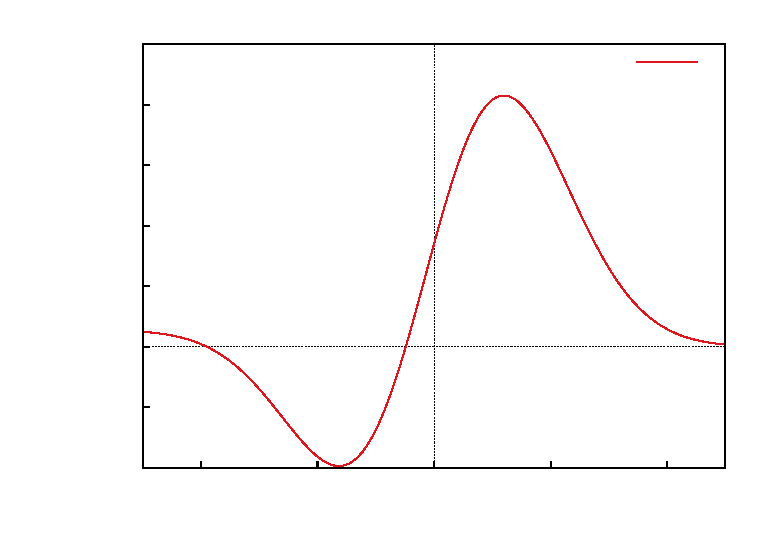
\includegraphics{./figures/elkc_exp_3D_gaussian_1}}%
    \gplfronttext
  \end{picture}%
\endgroup
}}\\
  \subfigure{\scalebox{0.5}{% GNUPLOT: LaTeX picture with Postscript
\begingroup
  \makeatletter
  \providecommand\color[2][]{%
    \GenericError{(gnuplot) \space\space\space\@spaces}{%
      Package color not loaded in conjunction with
      terminal option `colourtext'%
    }{See the gnuplot documentation for explanation.%
    }{Either use 'blacktext' in gnuplot or load the package
      color.sty in LaTeX.}%
    \renewcommand\color[2][]{}%
  }%
  \providecommand\includegraphics[2][]{%
    \GenericError{(gnuplot) \space\space\space\@spaces}{%
      Package graphicx or graphics not loaded%
    }{See the gnuplot documentation for explanation.%
    }{The gnuplot epslatex terminal needs graphicx.sty or graphics.sty.}%
    \renewcommand\includegraphics[2][]{}%
  }%
  \providecommand\rotatebox[2]{#2}%
  \@ifundefined{ifGPcolor}{%
    \newif\ifGPcolor
    \GPcolorfalse
  }{}%
  \@ifundefined{ifGPblacktext}{%
    \newif\ifGPblacktext
    \GPblacktexttrue
  }{}%
  % define a \g@addto@macro without @ in the name:
  \let\gplgaddtomacro\g@addto@macro
  % define empty templates for all commands taking text:
  \gdef\gplbacktext{}%
  \gdef\gplfronttext{}%
  \makeatother
  \ifGPblacktext
    % no textcolor at all
    \def\colorrgb#1{}%
    \def\colorgray#1{}%
  \else
    % gray or color?
    \ifGPcolor
      \def\colorrgb#1{\color[rgb]{#1}}%
      \def\colorgray#1{\color[gray]{#1}}%
      \expandafter\def\csname LTw\endcsname{\color{white}}%
      \expandafter\def\csname LTb\endcsname{\color{black}}%
      \expandafter\def\csname LTa\endcsname{\color{black}}%
      \expandafter\def\csname LT0\endcsname{\color[rgb]{1,0,0}}%
      \expandafter\def\csname LT1\endcsname{\color[rgb]{0,1,0}}%
      \expandafter\def\csname LT2\endcsname{\color[rgb]{0,0,1}}%
      \expandafter\def\csname LT3\endcsname{\color[rgb]{1,0,1}}%
      \expandafter\def\csname LT4\endcsname{\color[rgb]{0,1,1}}%
      \expandafter\def\csname LT5\endcsname{\color[rgb]{1,1,0}}%
      \expandafter\def\csname LT6\endcsname{\color[rgb]{0,0,0}}%
      \expandafter\def\csname LT7\endcsname{\color[rgb]{1,0.3,0}}%
      \expandafter\def\csname LT8\endcsname{\color[rgb]{0.5,0.5,0.5}}%
    \else
      % gray
      \def\colorrgb#1{\color{black}}%
      \def\colorgray#1{\color[gray]{#1}}%
      \expandafter\def\csname LTw\endcsname{\color{white}}%
      \expandafter\def\csname LTb\endcsname{\color{black}}%
      \expandafter\def\csname LTa\endcsname{\color{black}}%
      \expandafter\def\csname LT0\endcsname{\color{black}}%
      \expandafter\def\csname LT1\endcsname{\color{black}}%
      \expandafter\def\csname LT2\endcsname{\color{black}}%
      \expandafter\def\csname LT3\endcsname{\color{black}}%
      \expandafter\def\csname LT4\endcsname{\color{black}}%
      \expandafter\def\csname LT5\endcsname{\color{black}}%
      \expandafter\def\csname LT6\endcsname{\color{black}}%
      \expandafter\def\csname LT7\endcsname{\color{black}}%
      \expandafter\def\csname LT8\endcsname{\color{black}}%
    \fi
  \fi
  \setlength{\unitlength}{0.0500bp}%
  \begin{picture}(7200.00,5040.00)%
    \gplgaddtomacro\gplbacktext{%
      \csname LTb\endcsname%
      \put(1210,704){\makebox(0,0)[r]{\strut{} 0}}%
      \put(1210,1383){\makebox(0,0)[r]{\strut{} 2000}}%
      \put(1210,2061){\makebox(0,0)[r]{\strut{} 4000}}%
      \put(1210,2740){\makebox(0,0)[r]{\strut{} 6000}}%
      \put(1210,3418){\makebox(0,0)[r]{\strut{} 8000}}%
      \put(1210,4097){\makebox(0,0)[r]{\strut{} 10000}}%
      \put(1210,4775){\makebox(0,0)[r]{\strut{} 12000}}%
      \put(1888,484){\makebox(0,0){\strut{}-4}}%
      \put(2980,484){\makebox(0,0){\strut{}-2}}%
      \put(4073,484){\makebox(0,0){\strut{} 0}}%
      \put(5165,484){\makebox(0,0){\strut{} 2}}%
      \put(6257,484){\makebox(0,0){\strut{} 4}}%
      \csname LTb\endcsname%
      \put(176,2739){\rotatebox{90}{\makebox(0,0){\strut{}Surface area}}}%
      \put(4072,154){\makebox(0,0){\strut{}$\lset$}}%
    }%
    \gplgaddtomacro\gplfronttext{%
      \csname LTb\endcsname%
      \put(5816,4602){\makebox(0,0)[r]{\strut{}Theoretical}}%
    }%
    \gplbacktext
    \put(0,0){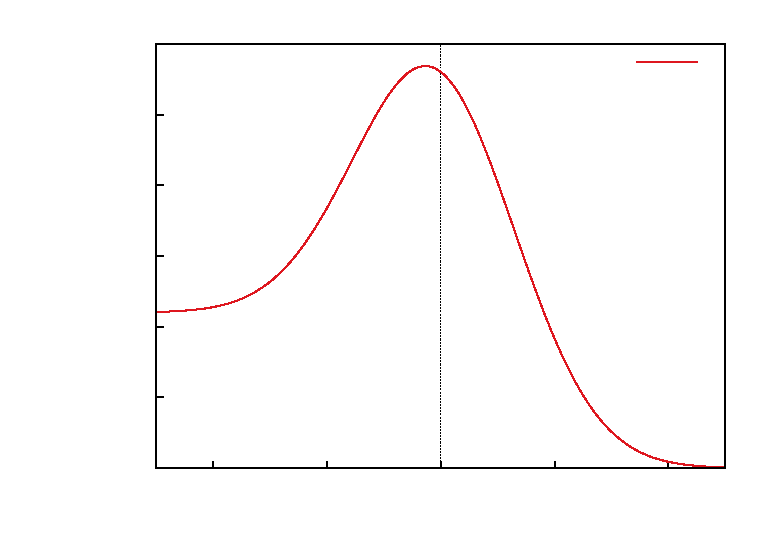
\includegraphics{./figures/elkc_exp_3D_gaussian_2}}%
    \gplfronttext
  \end{picture}%
\endgroup
}}\hspace{1.2cm}
  \subfigure{\scalebox{0.5}{% GNUPLOT: LaTeX picture with Postscript
\begingroup
  \makeatletter
  \providecommand\color[2][]{%
    \GenericError{(gnuplot) \space\space\space\@spaces}{%
      Package color not loaded in conjunction with
      terminal option `colourtext'%
    }{See the gnuplot documentation for explanation.%
    }{Either use 'blacktext' in gnuplot or load the package
      color.sty in LaTeX.}%
    \renewcommand\color[2][]{}%
  }%
  \providecommand\includegraphics[2][]{%
    \GenericError{(gnuplot) \space\space\space\@spaces}{%
      Package graphicx or graphics not loaded%
    }{See the gnuplot documentation for explanation.%
    }{The gnuplot epslatex terminal needs graphicx.sty or graphics.sty.}%
    \renewcommand\includegraphics[2][]{}%
  }%
  \providecommand\rotatebox[2]{#2}%
  \@ifundefined{ifGPcolor}{%
    \newif\ifGPcolor
    \GPcolorfalse
  }{}%
  \@ifundefined{ifGPblacktext}{%
    \newif\ifGPblacktext
    \GPblacktexttrue
  }{}%
  % define a \g@addto@macro without @ in the name:
  \let\gplgaddtomacro\g@addto@macro
  % define empty templates for all commands taking text:
  \gdef\gplbacktext{}%
  \gdef\gplfronttext{}%
  \makeatother
  \ifGPblacktext
    % no textcolor at all
    \def\colorrgb#1{}%
    \def\colorgray#1{}%
  \else
    % gray or color?
    \ifGPcolor
      \def\colorrgb#1{\color[rgb]{#1}}%
      \def\colorgray#1{\color[gray]{#1}}%
      \expandafter\def\csname LTw\endcsname{\color{white}}%
      \expandafter\def\csname LTb\endcsname{\color{black}}%
      \expandafter\def\csname LTa\endcsname{\color{black}}%
      \expandafter\def\csname LT0\endcsname{\color[rgb]{1,0,0}}%
      \expandafter\def\csname LT1\endcsname{\color[rgb]{0,1,0}}%
      \expandafter\def\csname LT2\endcsname{\color[rgb]{0,0,1}}%
      \expandafter\def\csname LT3\endcsname{\color[rgb]{1,0,1}}%
      \expandafter\def\csname LT4\endcsname{\color[rgb]{0,1,1}}%
      \expandafter\def\csname LT5\endcsname{\color[rgb]{1,1,0}}%
      \expandafter\def\csname LT6\endcsname{\color[rgb]{0,0,0}}%
      \expandafter\def\csname LT7\endcsname{\color[rgb]{1,0.3,0}}%
      \expandafter\def\csname LT8\endcsname{\color[rgb]{0.5,0.5,0.5}}%
    \else
      % gray
      \def\colorrgb#1{\color{black}}%
      \def\colorgray#1{\color[gray]{#1}}%
      \expandafter\def\csname LTw\endcsname{\color{white}}%
      \expandafter\def\csname LTb\endcsname{\color{black}}%
      \expandafter\def\csname LTa\endcsname{\color{black}}%
      \expandafter\def\csname LT0\endcsname{\color{black}}%
      \expandafter\def\csname LT1\endcsname{\color{black}}%
      \expandafter\def\csname LT2\endcsname{\color{black}}%
      \expandafter\def\csname LT3\endcsname{\color{black}}%
      \expandafter\def\csname LT4\endcsname{\color{black}}%
      \expandafter\def\csname LT5\endcsname{\color{black}}%
      \expandafter\def\csname LT6\endcsname{\color{black}}%
      \expandafter\def\csname LT7\endcsname{\color{black}}%
      \expandafter\def\csname LT8\endcsname{\color{black}}%
    \fi
  \fi
  \setlength{\unitlength}{0.0500bp}%
  \begin{picture}(7200.00,5040.00)%
    \gplgaddtomacro\gplbacktext{%
      \csname LTb\endcsname%
      \put(1210,704){\makebox(0,0)[r]{\strut{} 0}}%
      \put(1210,1213){\makebox(0,0)[r]{\strut{} 5000}}%
      \put(1210,1722){\makebox(0,0)[r]{\strut{} 10000}}%
      \put(1210,2231){\makebox(0,0)[r]{\strut{} 15000}}%
      \put(1210,2740){\makebox(0,0)[r]{\strut{} 20000}}%
      \put(1210,3248){\makebox(0,0)[r]{\strut{} 25000}}%
      \put(1210,3757){\makebox(0,0)[r]{\strut{} 30000}}%
      \put(1210,4266){\makebox(0,0)[r]{\strut{} 35000}}%
      \put(1210,4775){\makebox(0,0)[r]{\strut{} 40000}}%
      \put(1888,484){\makebox(0,0){\strut{}-4}}%
      \put(2980,484){\makebox(0,0){\strut{}-2}}%
      \put(4073,484){\makebox(0,0){\strut{} 0}}%
      \put(5165,484){\makebox(0,0){\strut{} 2}}%
      \put(6257,484){\makebox(0,0){\strut{} 4}}%
      \csname LTb\endcsname%
      \put(176,2739){\rotatebox{90}{\makebox(0,0){\strut{}Volume}}}%
      \put(4072,154){\makebox(0,0){\strut{}$\lset$}}%
    }%
    \gplgaddtomacro\gplfronttext{%
      \csname LTb\endcsname%
      \put(5816,4602){\makebox(0,0)[r]{\strut{}Experimental}}%
      \csname LTb\endcsname%
      \put(5816,4382){\makebox(0,0)[r]{\strut{}Theoretical}}%
    }%
    \gplbacktext
    \put(0,0){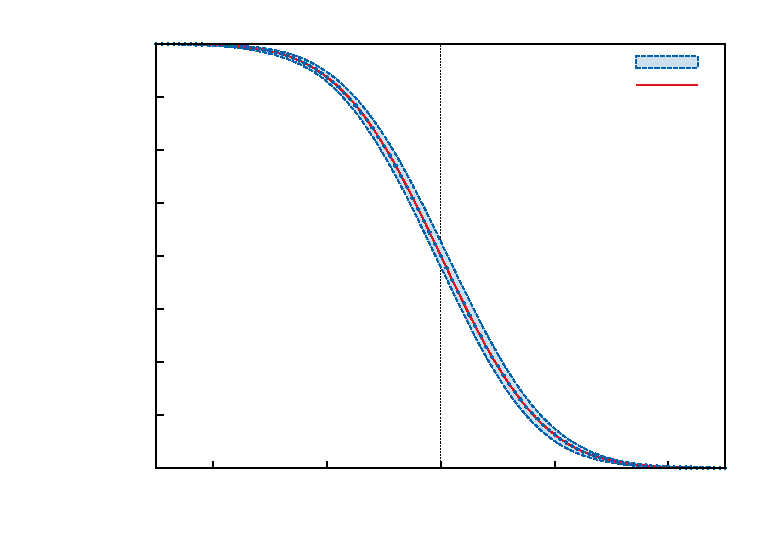
\includegraphics{./figures/elkc_exp_3D_gaussian_3}}%
    \gplfronttext
  \end{picture}%
\endgroup
}}\\
  \caption{Expectation of LKC for $\PRF=100\times 20 \times 20$, $\mean=0.0$, $\std^2=2$, $\Lc=2$, and $\HS=\uinf$ (gaussian distribution with tail hitting set) in 3D. Experimental results are calculated over $100$ realizations.}
\end{figure}

\end{document}
